\chapter{Delegation}

An important design decision when modeling data is how many Java classes to use to represent an entity. The choices made at this design stage can impact memory costs significantly. At one extreme, all of the attributes of an entity may be stored in a single class. At the other extreme, a main entity class may delegate many of its attributes to other classes, resulting in a fine-grained design. Delegation is a very popular pattern because of the flexibility it provides. It is also one of the few ways Java allows you to reuse existing classes. Yet, overly fine-grained data models can result in poor memory health. This chapter explains how to evaluate the granularity of a design design from a memory perspective. It begins with the costs of basic objects, and shows how they add in real applications.
  
\section{The Cost of Objects}
\label{sec:CostOfObjects}

There is no Java library method that returns the size of an object. This is by design. Unlike systems languages like C, a Java programmer is not supposed to know either the size of an object or how it is laid out in memory. The JVM, not the programmer, manages storage, and the JVM has freedom to implement its own policy. However, knowing the sizes of objects is necessary for understanding memory requirements and scalability. Fortunately, it is not hard to estimate the size of an object, and a good estimate of the most prevelant classes is usually sufficient for making intelligent design choices.  You need to know just a few basics, starting with the size of the Java primitive types. These are given in Table~\ref{tab:primitive-sizes}.
\begin{table}
  \centering
 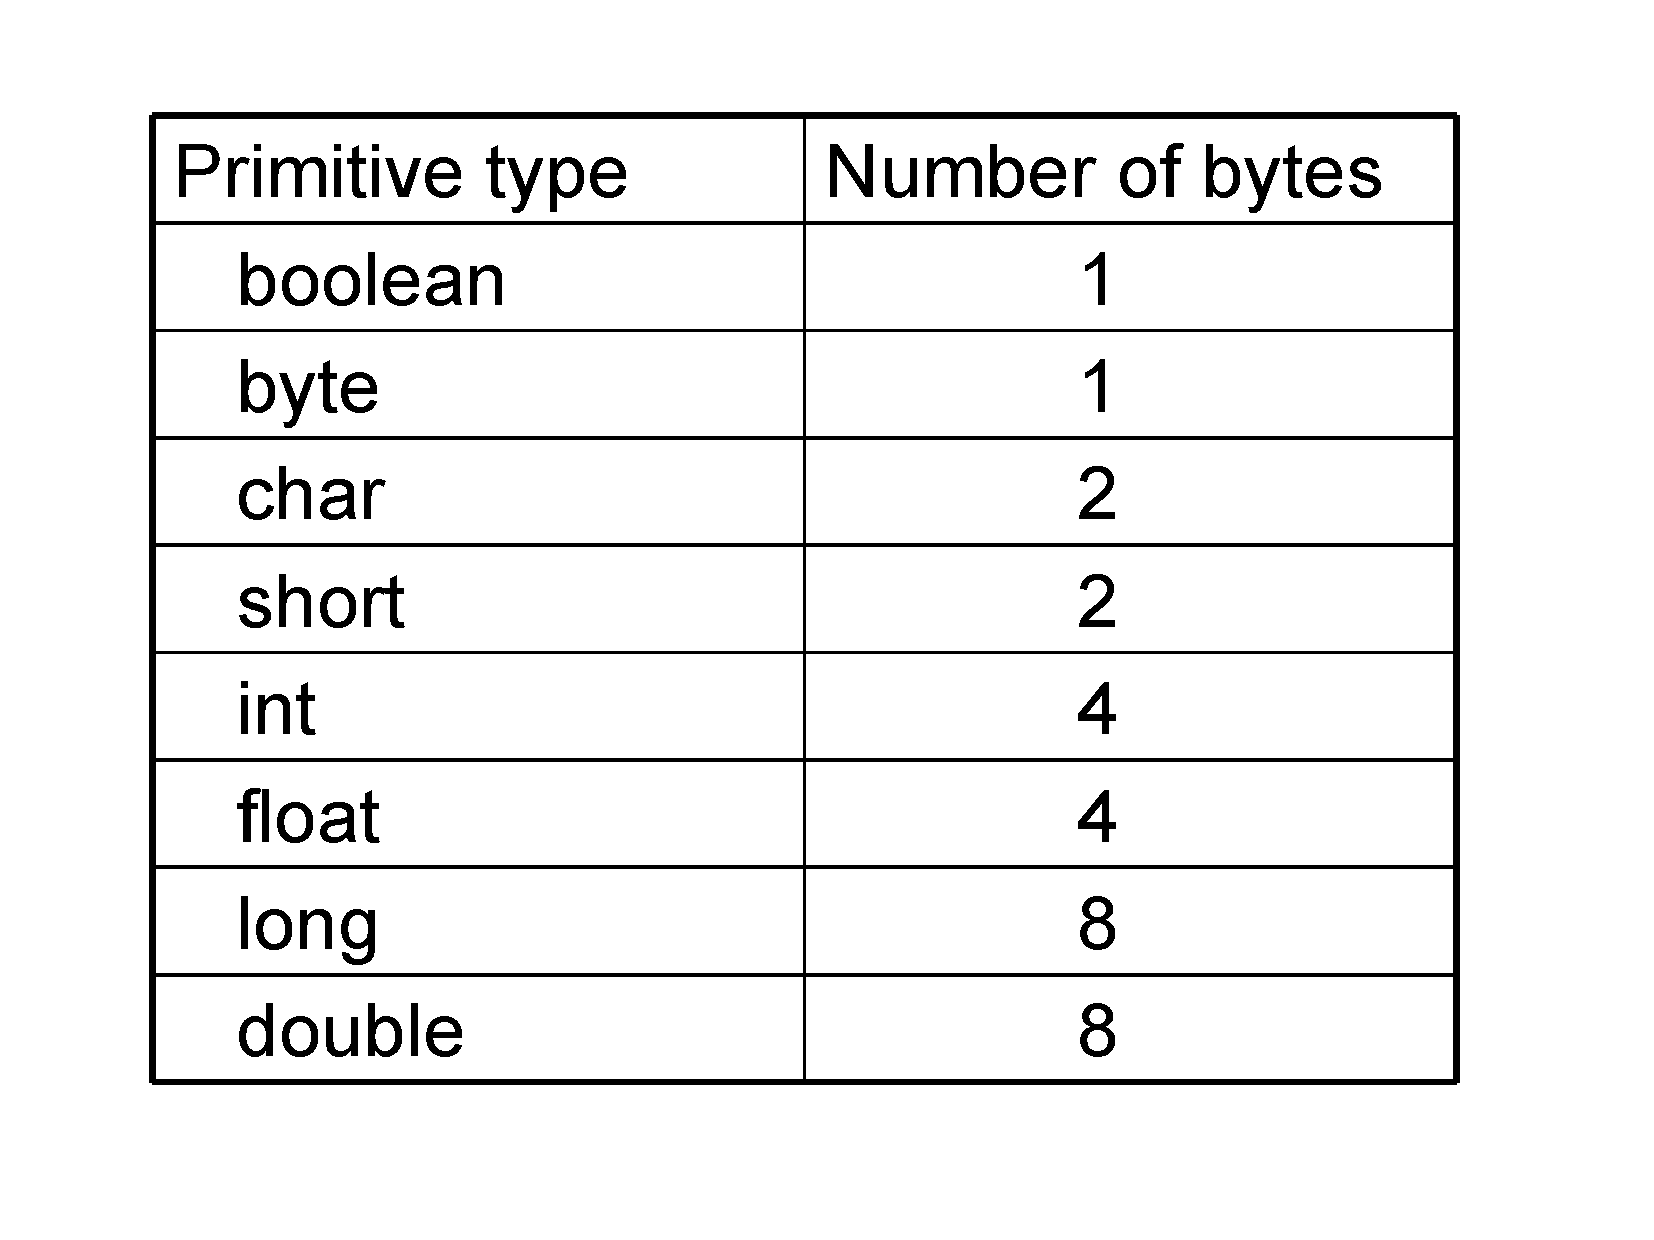
\includegraphics[width=.50\textwidth]{Figures/chapter4/primitive-byte-sizes.pdf}
 % 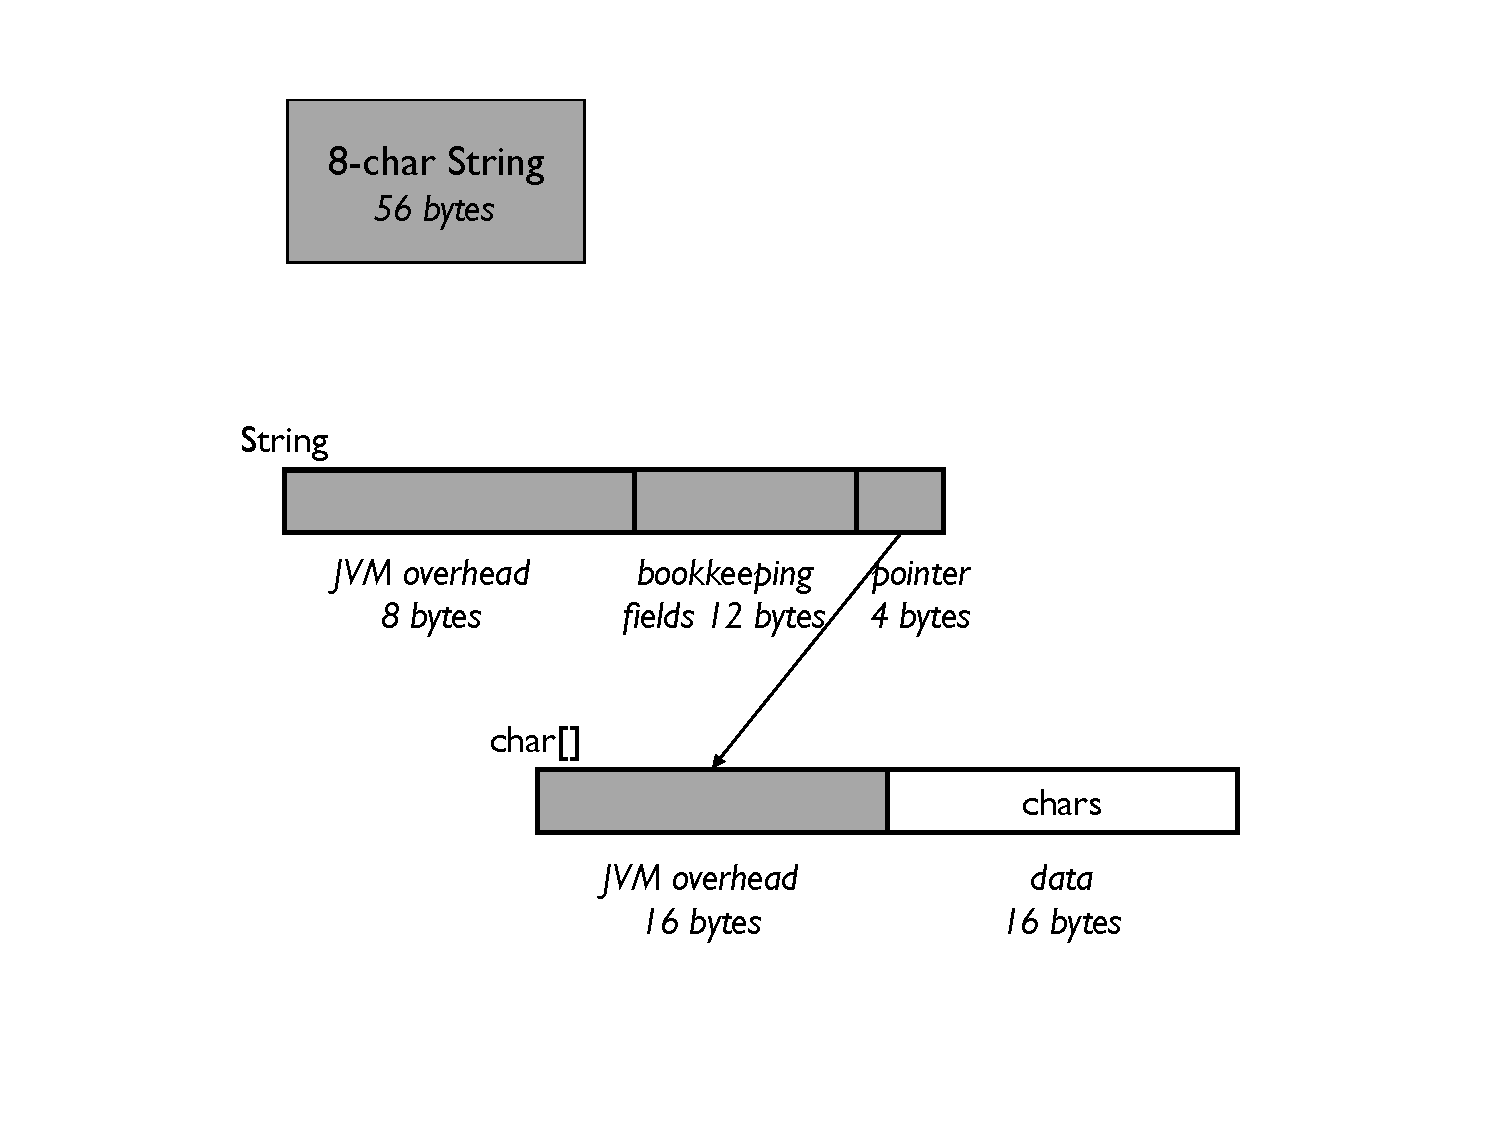
\includegraphics{eight-char-string}
  \caption{The sizes of Java primitive types}
  \label{tab:primitive-sizes}
\end{table}

Objects are bigger than the sum of their fields. First, the JVM allocates a header with each object that stores information such as the object's class and various flags. For array objects, the header has an additional integer to store the number of array elements. Secondly, the hardware imposes alignment costs. The hardware may require 2-byte, 4-byte, or 8-byte alignment, depending on the type of the data. For example, integers are usually aligned on a 4-byte boundary, and some hardware might require a double to be aligned on an 8-byte boundary. Popular JVMs impose additional alignment requirements. This overhead is significant, especially if the object does not have much data in it.

Object header sizes and alignment costs vary depending on the JVM. Table~\ref{tab:object-overhead} gives the costs for both the SUN Java 6 (update 14) JVM and the IBM Java 6 (J9 SR4) JVM. These costs are for 32-bit architectures. It is important to keep in mind that these costs are for specific JVM releases only, and are subject to change in future releases.
\begin{table}
  \centering
 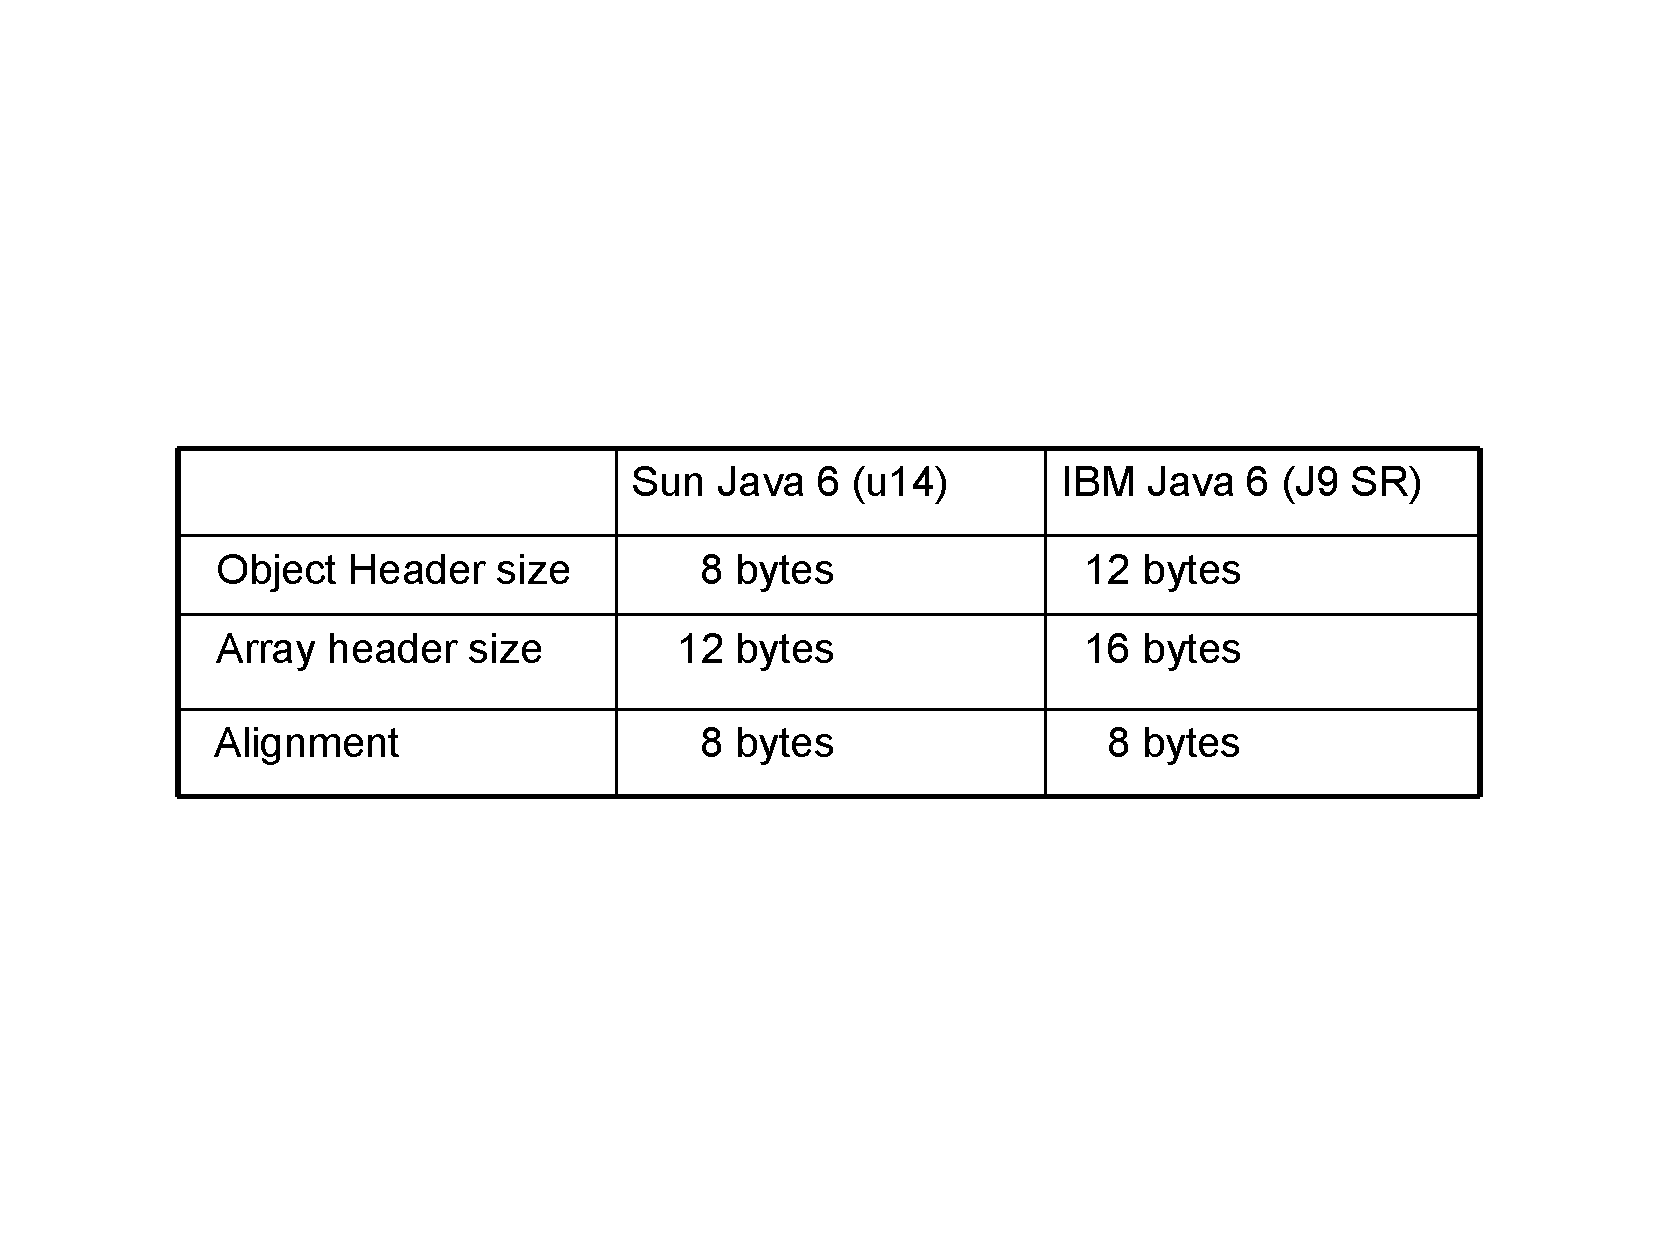
\includegraphics[width=.70\textwidth]{Figures/chapter4/object-overhead.pdf}
 % 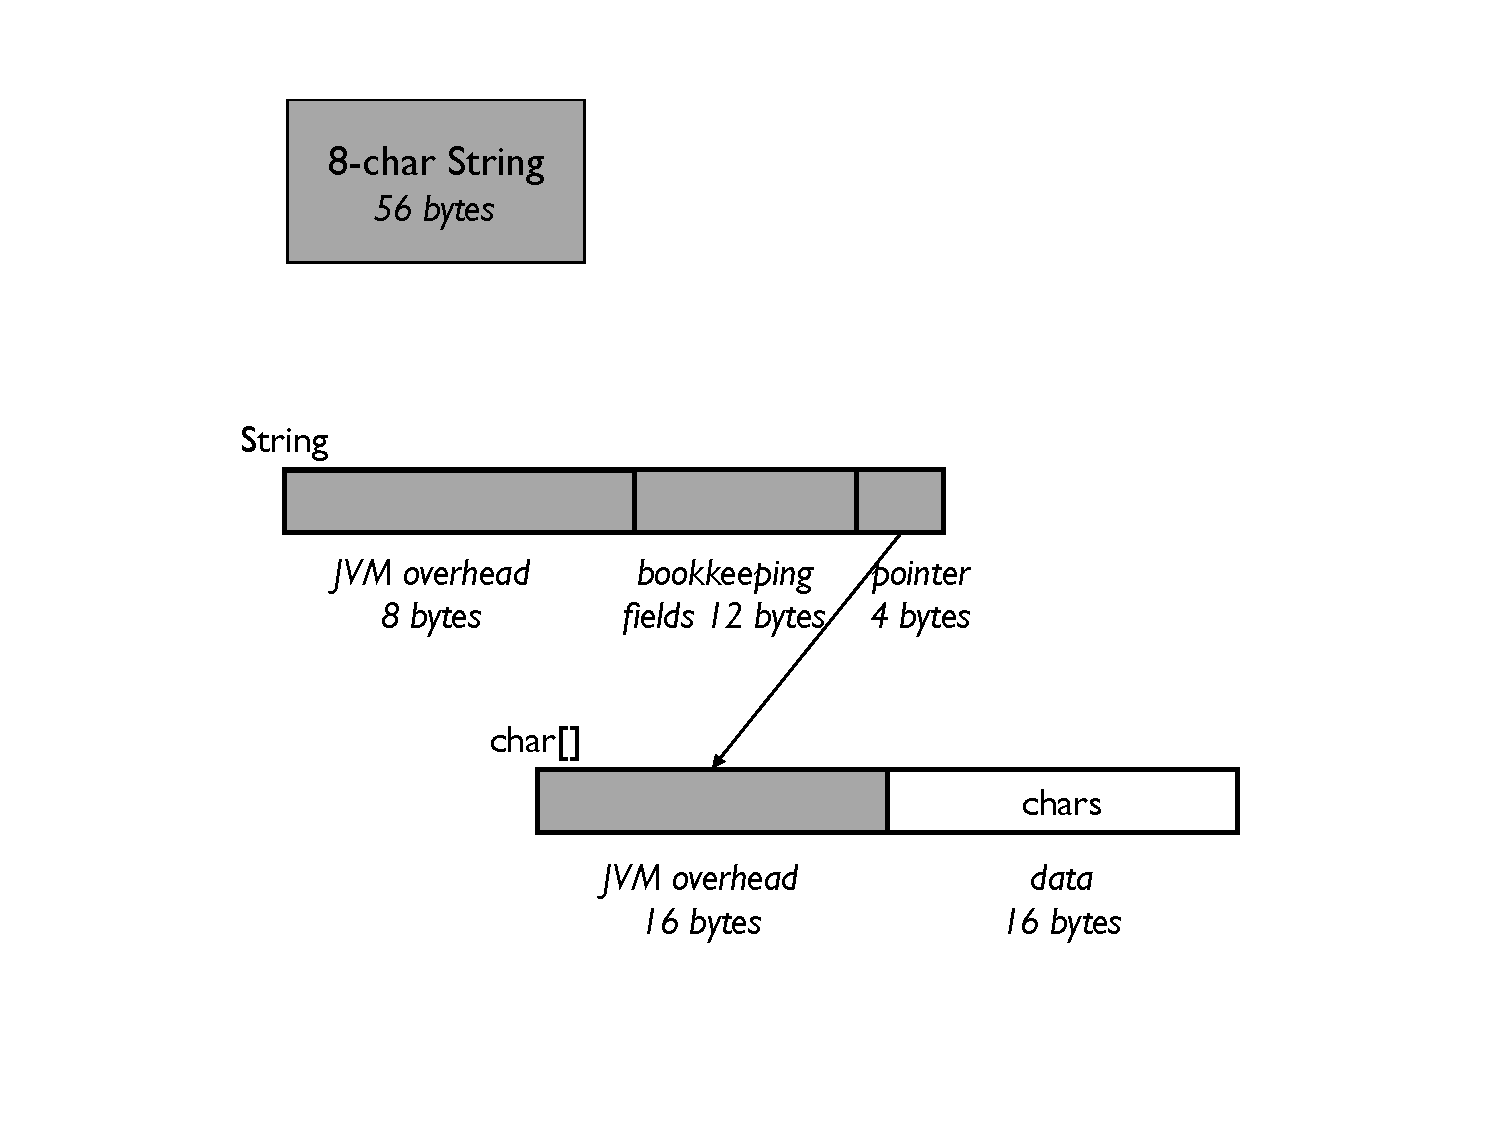
\includegraphics{eight-char-string}
  \caption{The sizes of boxed scalar objects.}
  \label{tab:object-overhead}
\end{table} 
   %The Sun JVM allocates 8 bytes per object header, and the IBM JVM allocates 12 bytes per header. 
 
Boxed scalars, which are objects with a single primitive data type field, are the simplest kind of  object. For both the Sun and IBM JVMs, a boxed scalar is at least 16 bytes. Since both JVMs allocate objects on 8-byte boundaries, the size of an object must be a multiple of 8. Table~\ref{tab:boxed-scalar-sizes} gives the sizes of boxed scalars.

\begin{table}
  \centering
 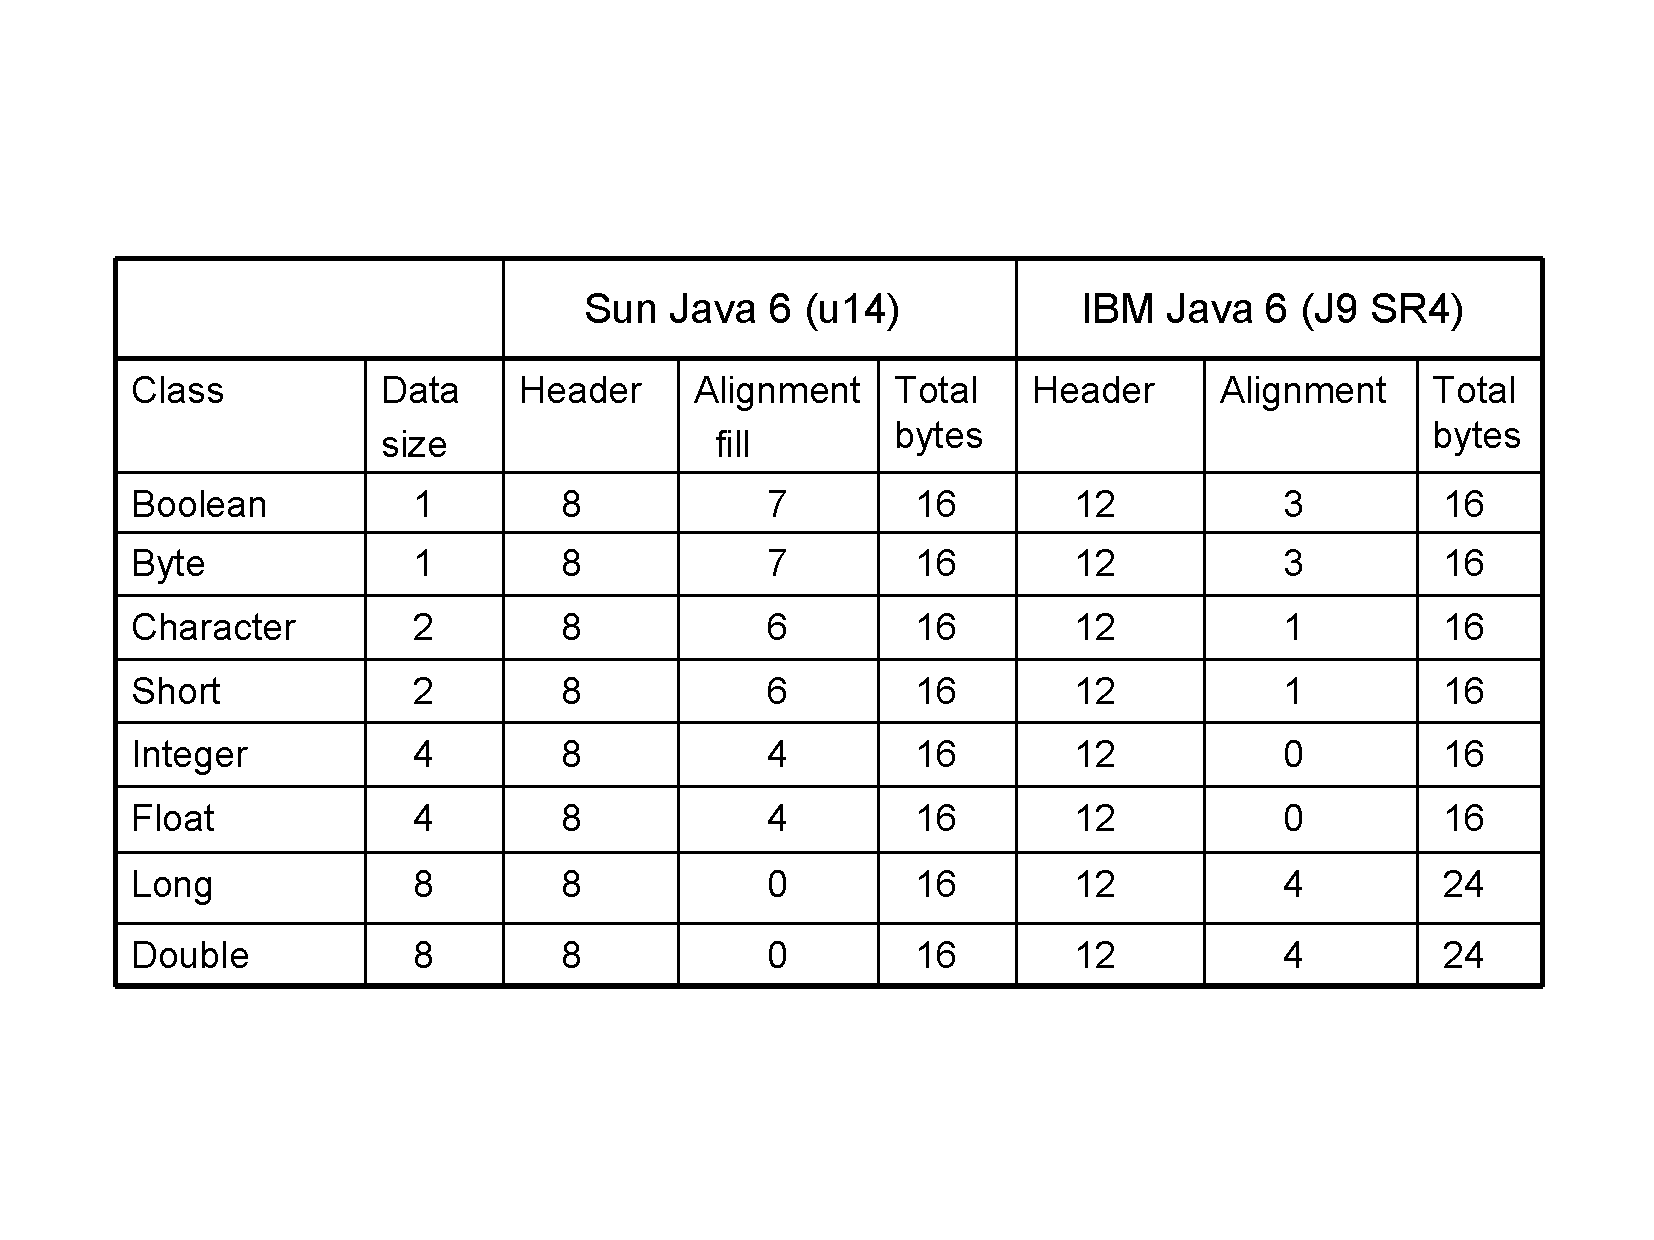
\includegraphics[width=.70\textwidth]{Figures/chapter4/boxed-scalar-sizes.pdf}
 % 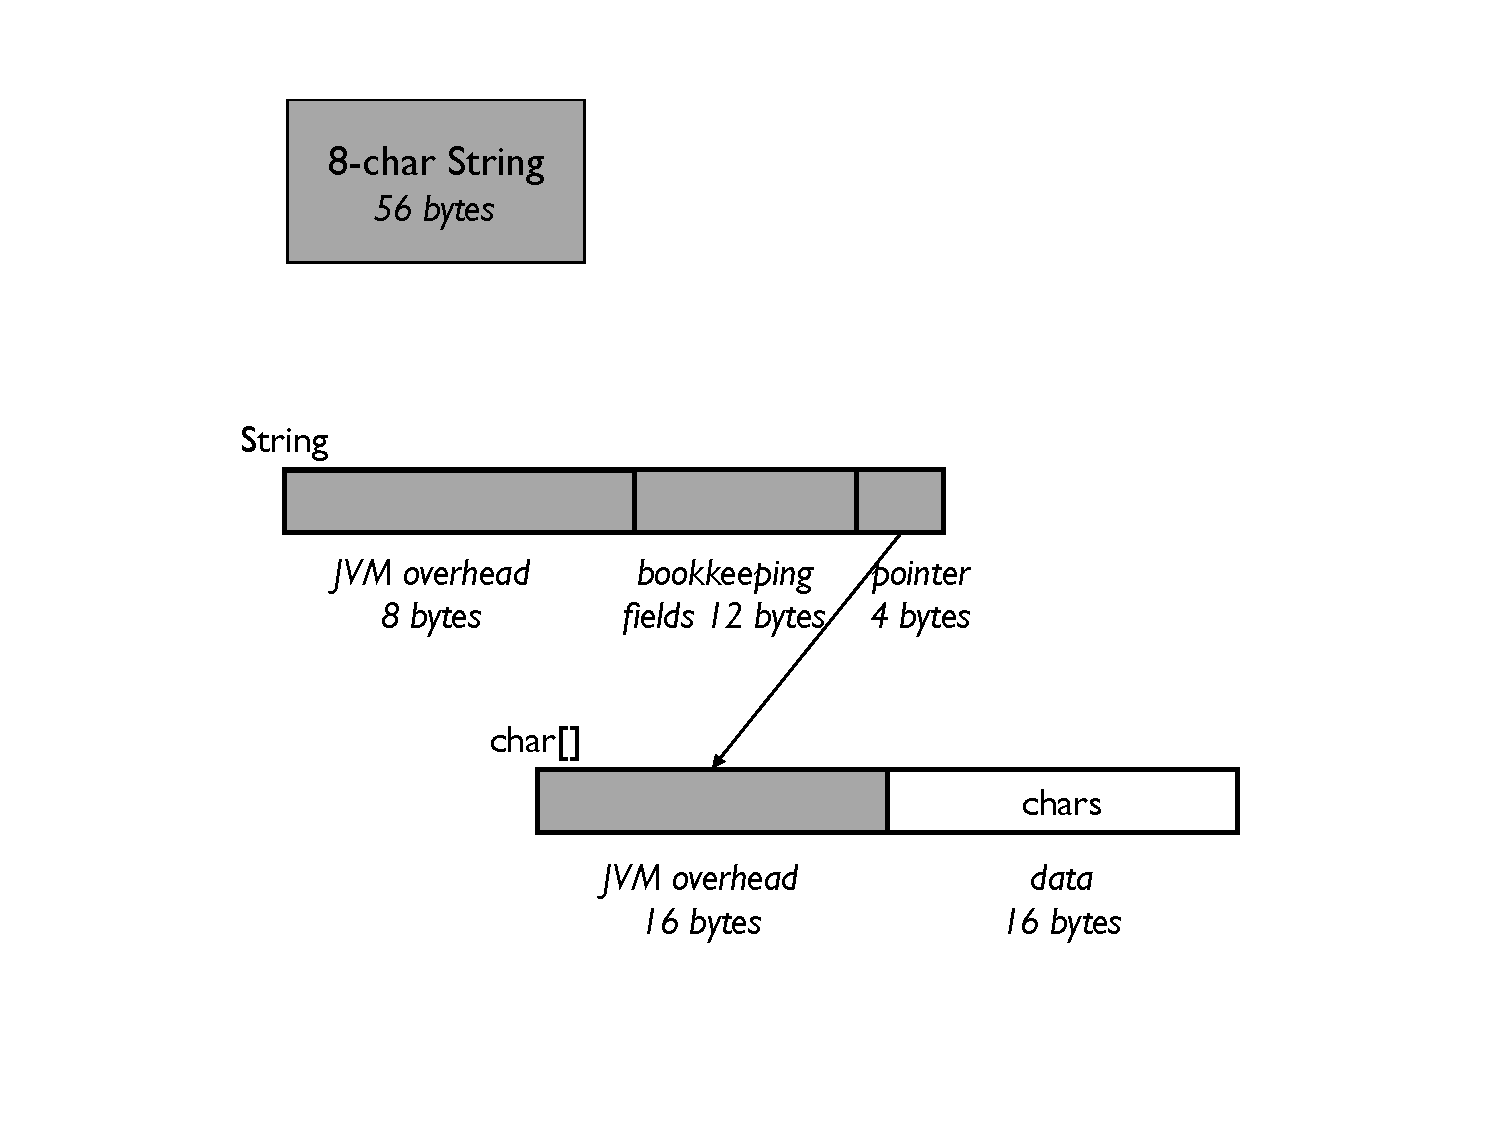
\includegraphics{eight-char-string}
  \caption{The sizes of boxed scalar objects.}
  \label{tab:boxed-scalar-sizes}
\end{table} 
Just like for boxed scalars, the minimum  size of any object can be obtained by summing the size of the header and the data, and then rounding it up to the nearest multiple of 8 (which JVM???).  
 
\callout{callout:minimum-size-estimation-rule}{Estimating Minimum Size}{
MORE SCHEMATIC...
    Let \textit{Header} be the size of an object header required by the JVM, and \textit{Alignment} be the object alignment. That is, every object must be allocated at an address which is a multiple of $Alignment$. To estimate the minimum size of an object 1) sum up the sizes of all of its fields, including fields from superclasses, 2) add \textit{Header} to this sum, and 3) round the result up to the next multiple of \textit{Alignment}. The estimate is exact if the JVM packs and rearranges fields to fit into the smallest space. Otherwise, the actual size can be bigger than the estimated size.
}

\begin{example}[Simple employee class.]
Consider an \texttt{Employee} class with all primitive fields:

\ttfamily
\begin{verbatim} 

			class Employee {
        int hoursPerWeek;        // 4 bytes
        boolean exempt;          // 1 byte
        double salary;           // 8 bytes
        char jobCode;            // 2 bytes
        int yearsOfService;      // 4 bytes
			}
\end{verbatim}
\normalfont
Assume both \textit{Header} and \textit{Alignment} are 8 bytes. To apply the minimum-size rule to \texttt{Employee} first add the primitive field sizes 4+1+8+2+4 (=19), then add in the header size 8 (=27), and then round to the next multiple of 8. The result is 32 bytes.  If the header is 12 bytes, the estimated size is also 32 bytes, since 19+12 is 31, which again rounds up to 32. 
\end{example}

How accurate are these estimates for the two JVMs?  For the Sun JVM, an \texttt{Employee} object is exactly 32 bytes. The minimum-size estimate rule works well here, since the Sun JVM does a good job packing fields. For the IBM JVM, the real size of an \texttt{Employee} object is 40 bytes, not 32. The IBM JVM does not pack fields that are less than 4 bytes. In other words, the IBM JVM aligns all fields on 4 byte boundaries. When an object has several fields that are less than 4 bytes, such as booleans and chars, the minimum-size estimate rule can underestimate its size. 

A modified version of the minimum-size estimate rule, where fields are never less than 4 bytes, works better for the IBM JVM. To apply this modified rule to \texttt{Employee}, first add the field sizesa 4+4+8+4+4 (=24), add in the IBM JVM header size 12 (=36), and then round up the result to 40 bytes.
\ttfamily
\begin{verbatim} 

			class Employee {
        int hoursPerWeek;        // 3 bytes
        boolean exempt;          //  byte
        double salary;           // 8 bytes
        char jobCode;            // 2 bytes
        int yearsOfService;      // 4 bytes
			}
\end{verbatim}
\normalfont

\callout{callout:word-aligned-estimation-rule}{Word-Aligned Estimate Rule}{
    Let \textit{Header} be the size of an object header required by the JVM, and \textit{Alignment} be the object alignment. To estimate the size of an object 1) sum up the sizes of all of its fields including superclass fields, \textsl{assuming each field is aligned on a 4-byte boundary} 2) add \textit{Header} to this sum, and 3) round the result up to the next multiple of \textit{Alignment}. 
}

Understanding the memory costs starts with understanding the cost of important classes.  These are the classes that will be instantiated the most, that will have the most impact on scalability. The bloat factor, the percentage of memory overhead, is an other metric that helps to understand how much room there is for improvement. If the bloat factor is very high, then it should be possible to find a more efficient representation. The question is, what is too high?  
In this example, the bloat factor is 46\% for the Sun JVM, and 53\% for the IBM JVM. The overhead comes completely from object header and alignment. For such a simple object, you really can not do any better than this. In fact, for Java programs in general, any  bloat factor less than 50\% is extremely good.

For this purpose of evaluating design alternatives, a good estimate is completely adequate. If you need the exact sizes of an objects, you can get them from HPROF heap snapshots. The \texttt{jmap} utility that comes with the Sun JVM distribution writes an HPROF heap dump:
\ttfamily
\begin{verbatim} 
      jmap -dump:format=a,file=outputfile <pid of jvm process> 
\end{verbatim}
If you do not have \texttt{jmap}, you can enable the HPROF agent using the command line option: 
\ttfamily
\begin{verbatim} 
      -agentlib:hprof=heap=dump,format=a,file=outputfile
\end{verbatim}
\normalfont
Sending a signal to the JVM process produces a heap snapshot in \textit{outputfile}.


\section{The Cost of Delegation}

The \texttt{Employee} class is not a very realistic example, since it has only primitive fields. Usually, a class has fields that are objects.  In Java, an object field is implemented as a \textit{delegated} object, that is, as a separate object pointed to by the owner object. On 32-bit architectures, a pointer is 4 bytes. You can estimate the size of any object using the estimate rules in Section~\ref{sec:CostOfObjects}, plugging in 4 bytes for each object field. Unless otherwise stated, the following examples assume the Sun JVM. 
\begin{example}[Employee class with object fields]
Here is a more realistic \texttt{Employee} class, with several object fields. An employee now has a name, which is a \texttt{String}, and a start date, which is a \texttt{Date}. The type of \texttt{salary} has been changed from \texttt{double} to \texttt{BigDecimal}. \texttt{BigDecimal} avoids potential roundoff errors.
\ttfamily
\begin{verbatim} 
			class Employee {
        int hoursPerWeek;
        String name;
        BigDecimal salary;
        Date startDate;
        boolean exempt;
        char jobCode;
        int yearsOfService;
			}
\end{verbatim}
\normalfont
To estimate the size of this \texttt{Employee} object, add the field sizes 4+4+4+4+1+2+4 (=23), add in 8 bytes for the header (=31), and then round this up to 32 bytes. 
\end{example}

While an instance of the \texttt{Employee} class is a single 32 byte object, an instance of an entire employee entity, including name, salary, and start date consists of five objects. Two of these objects are used to store the name \texttt{String}. Recall from Section~\ref{sec:bloat-def} that a string is represented by a wrapper \texttt{String} object and a \texttt{char} array. The memory layout for a specific employee ``John Doe" is shown in Figure~\ref{fig:employee-status}. 
 \begin{figure}
  \centering
 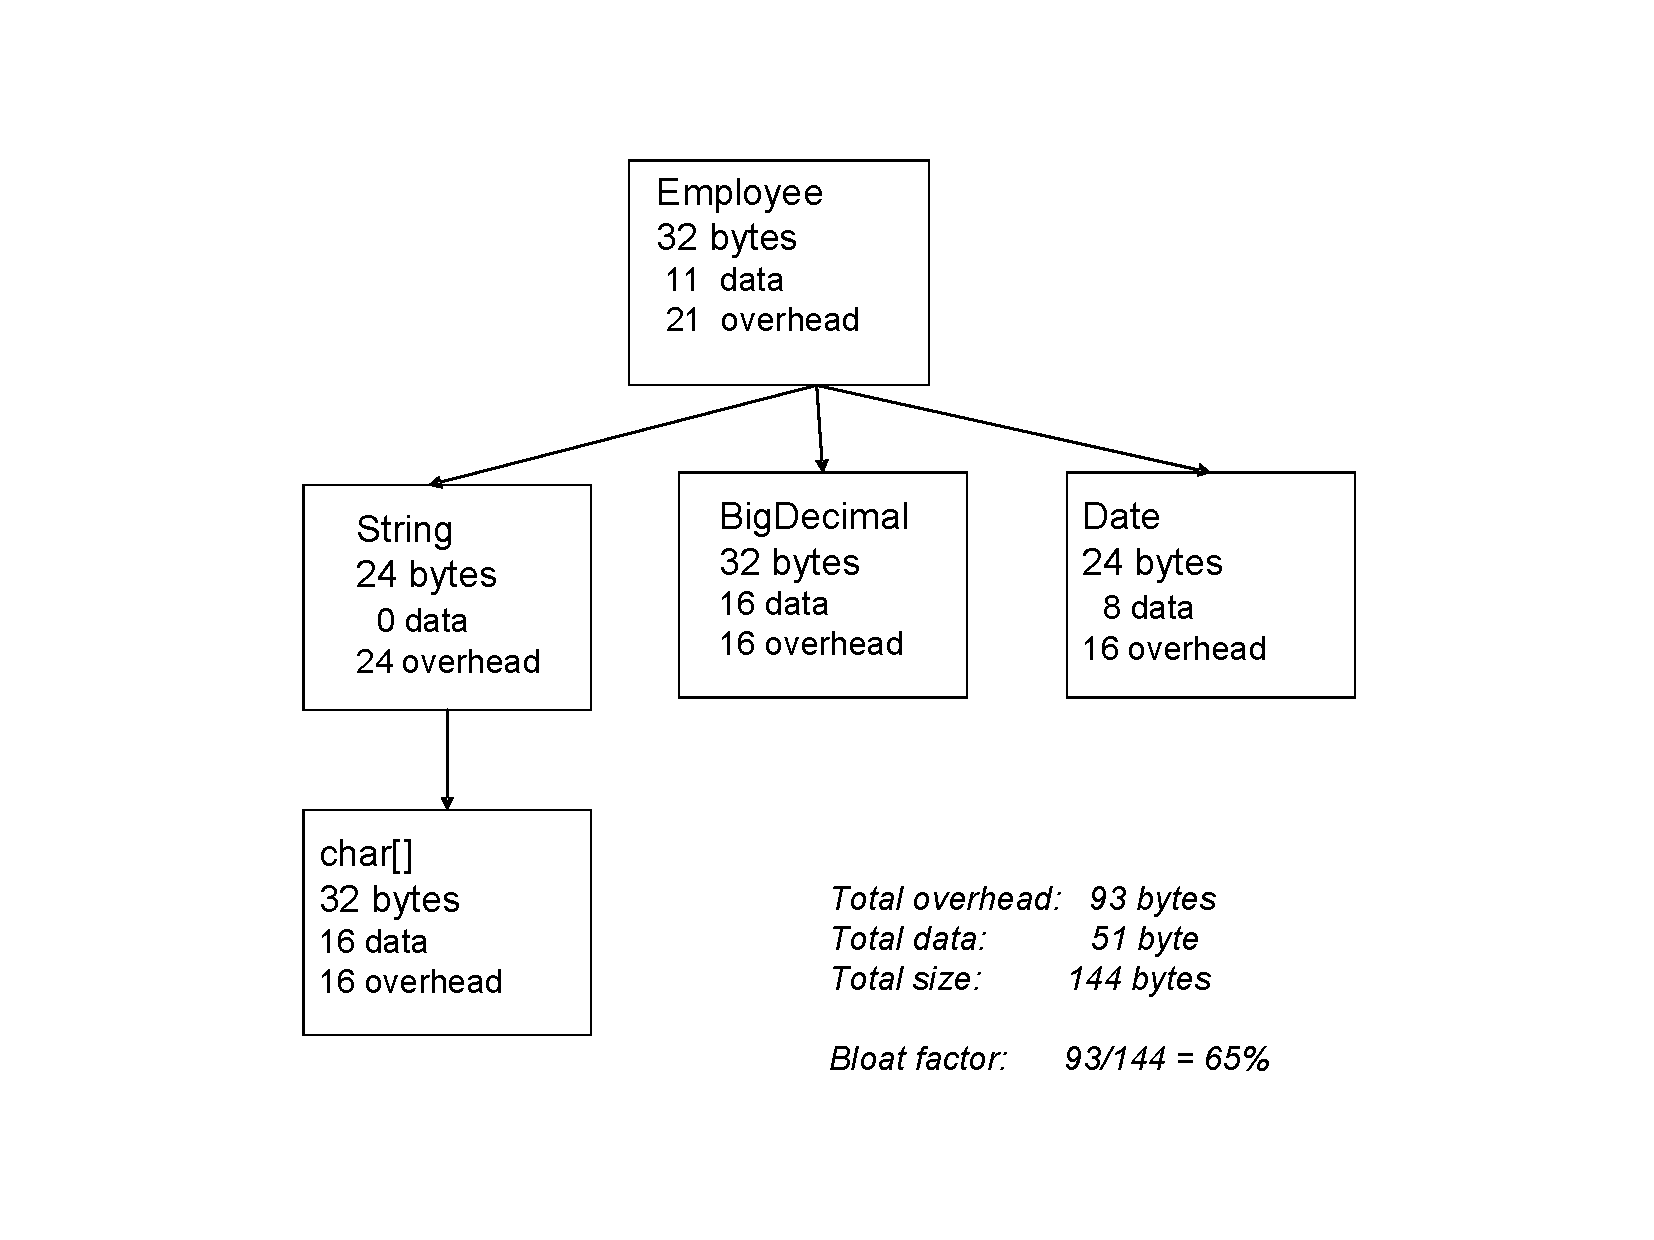
\includegraphics[width=.60\textwidth]{Figures/chapter4/employee-status.pdf}
 % 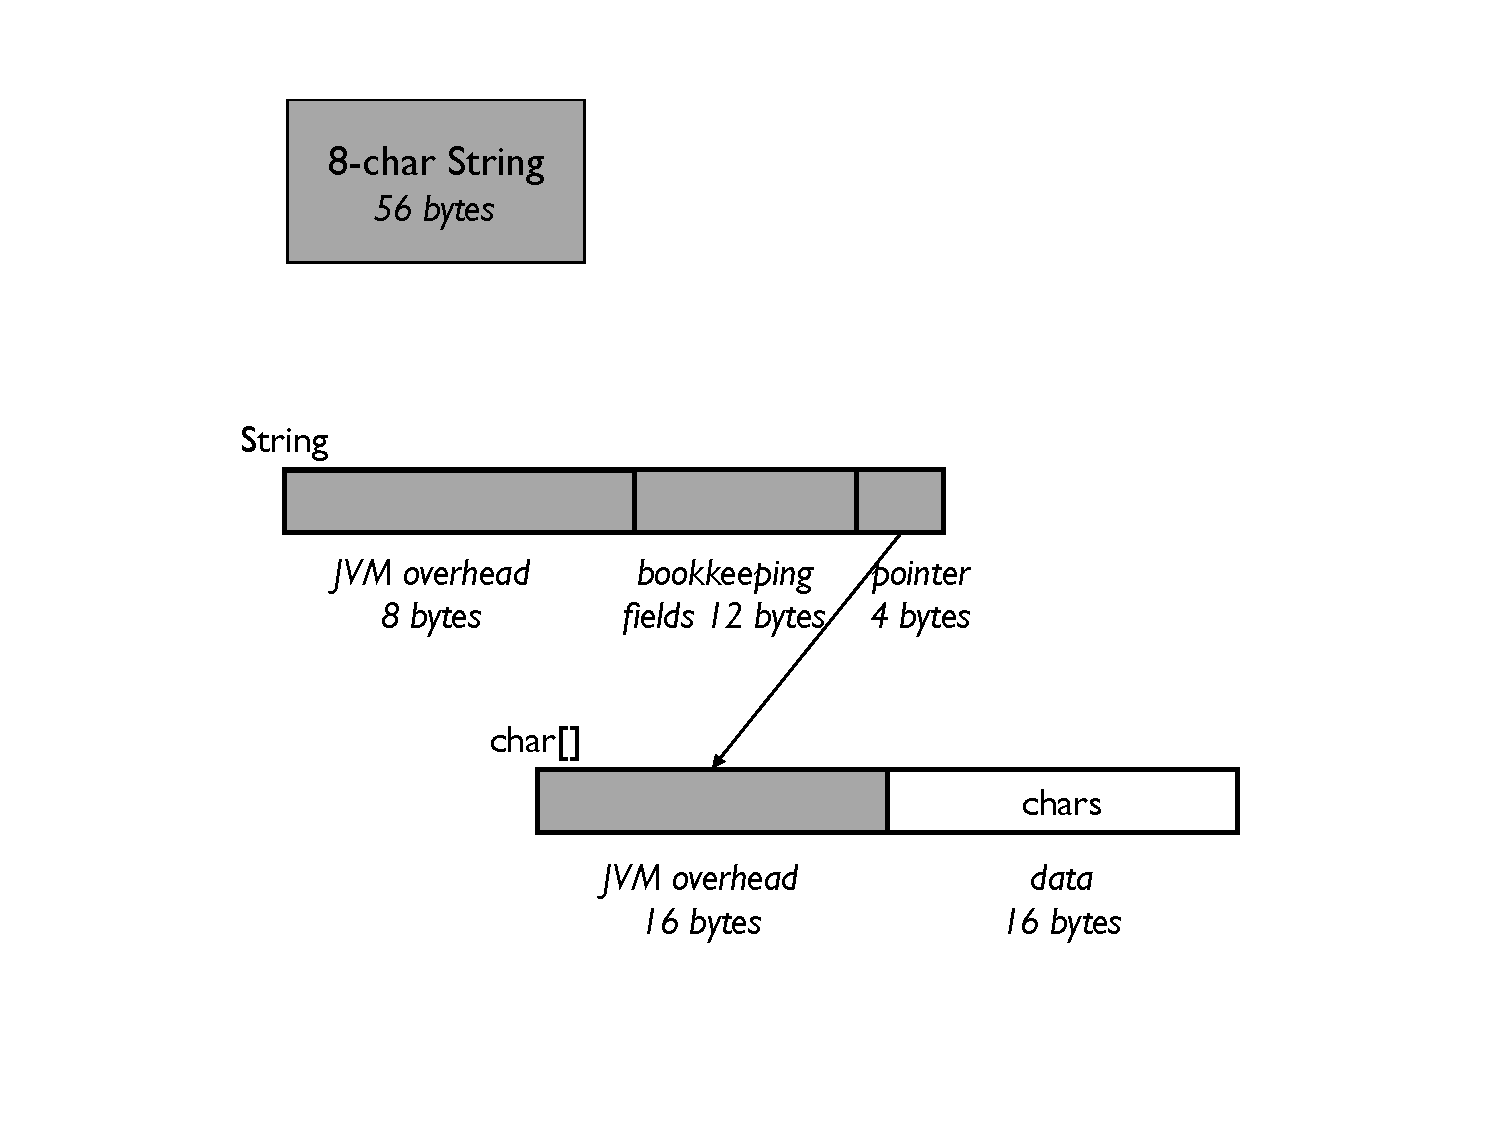
\includegraphics{eight-char-string}
  \caption{The memory layout for an employee ``John Doe"}
  \label{fig:employee-status}
\end{figure}

A comparion of this mult-object employee with the original \texttt{Employee} object in Section~\cite{CostOfObects} shows that the size has increased from 32 to 144 bytes, and the bloat factor has increased from 46\% to 65\%. There is more information stored in the new version, so it is no surprise that it is bigger. The increase in the bloat factor is more significant. Delegation increases memory bloat. Delegation introduces additional object headers, a pointer for each delegated object, and empty pointer slots for unitialized object fields. Delegation may also force additional alignment costs, since each new delegated object has to be aligned to an 8-byte boundary. 

In the spirit of keeping things simple, Java does not allow you to nest objects inside other objects, to build a single object out of other objects. You cannot nest an array inside an object, and you cannot store objects directly in an array.  You can only point to other objects. Even the basic data type \texttt{String} consists of two objects. This means that delegation is pervasive in Java programs, and it is difficult to avoid a high level of delegation overhead. Single inheritance is the only language feature that can be used instead of delegation to compose two object, but single inheritance has limited flexibility.  In contrast, C++ has many different ways to compose objects. C++ has single and multiple inheritance, union types, and variation. C++ allows you to have \texttt{struct} fields, you can put arrays inside of structs, and you can also have an array of structs.  

Because of the design of Java, there is a basic delegation cost that is hard to eliminate. It is the cost of object-oriented programming in Java. While it is hard to avoid this basic delegation cost, it is important not to make things a lot worse, as discussed in the next section. 

\section{Fine-Grained Data Models}
\label{fine-grained-data-models}

The Java language makes it hard to avoid delegation. Programmer choices also impact delegation costs.  The current software engineering culture tends to promote delegation, and for good reasons. Delegation provides a loose coupling of objects, making refactoring and reuse easier. Replacing inheritance by delegation is often recommended, especially if the base class has extra fields and methods that the subclass does not need. In languages with single inheritance, once you have used up your inheritance slot, it becomes hard to refactor your code. Therefore, delegation can be more flexible than inheritance for implementing polymorphism. However, overly fine-grained data models can be expensive both in execution time and memory space. 

There is no simple rule that can always be applied to decide when to use delegation. Each situation has to be evaluated in context, and there may be tradeoffs among different goals. To make an informed decision, it is important to know what the costs are.

\begin{example}[Employee emergency contact] 
Suppose an emergency contact is needed for each employee. An emergency contact is a person along with a preferred method to reach her.  The preferred method can be email, cell phone, work phone, or home phone. All contact information for the emergency contact person must be stored, just in case the preferred method does not work in an actual emergency. 
\end{example}
Here are class definitions for an emergency contact, written in a highly delegated style that is not uncommon in real applications. 

\ttfamily
\begin{verbatim} 
			class Employee {
        ...
        EmergencyContact contact;
			}
			
			class EmergencyContact {
        ContactPerson contact;
        ContactMethod preferredContact;
			}
			
			class ContactPerson {
        String name;
        String relation;
        EmailAddress email;
        PhoneNumber phone;
        PhoneNumber cell;
        PhoneNumber work;
			}
			
			class ContactMethod {
        ContactPerson owner;
			}
			
			class PhoneNumber extends ContactMethod {
			  byte[] phone;
			}
			
			class EmailAddress extends ContactMethod {
        String address;
			}
			
			
\end{verbatim}
\normalfont
 \begin{figure}
  \centering
 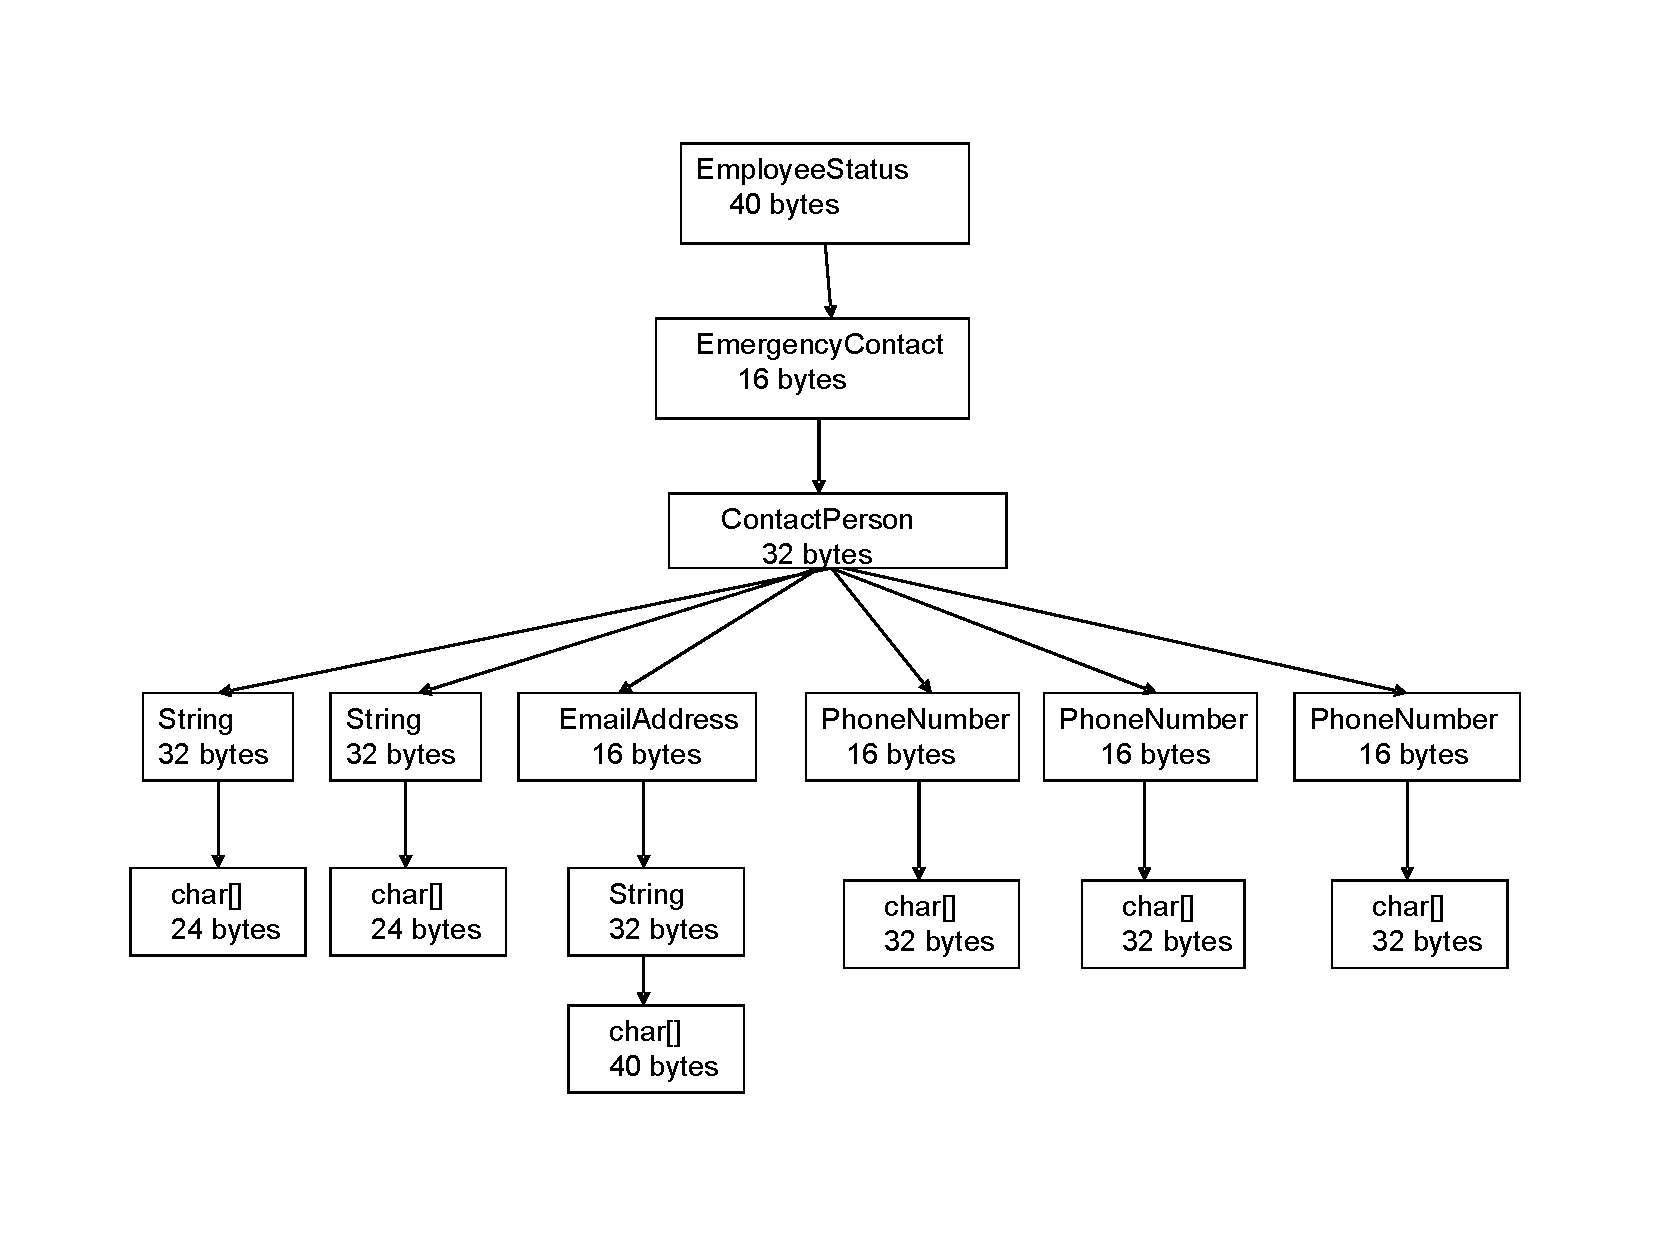
\includegraphics[width=.70\textwidth]{Figures/chapter4/employee-status-fine-grained.pdf}
 % 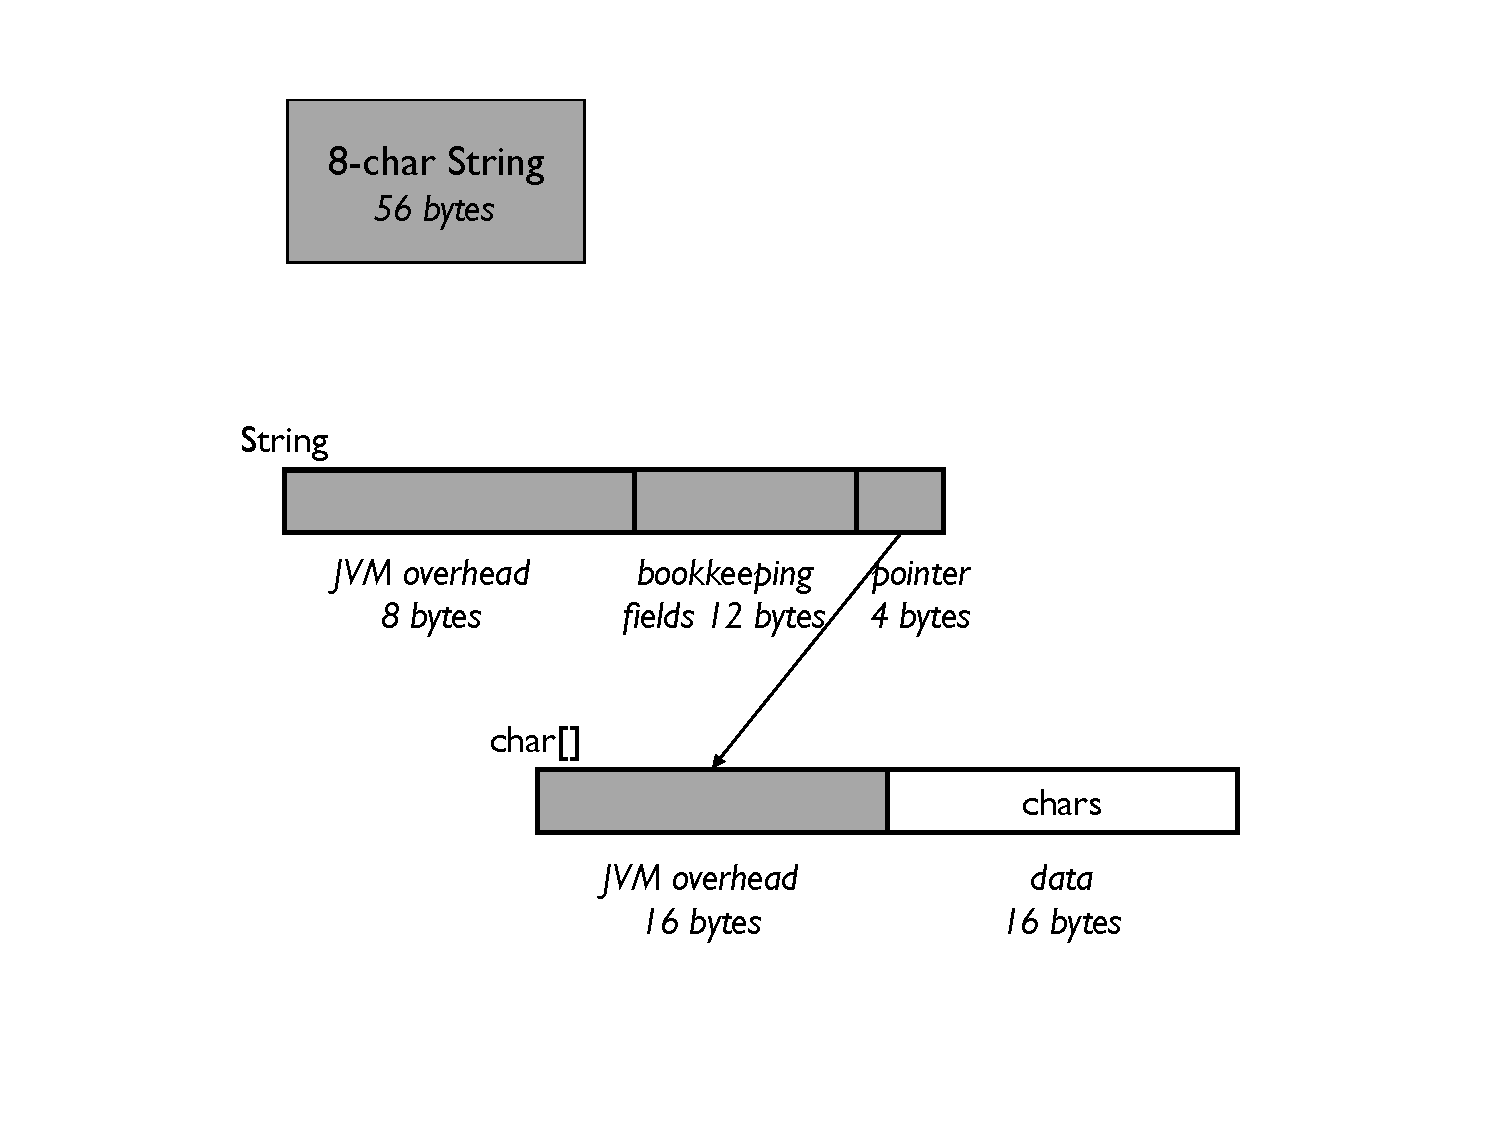
\includegraphics{eight-char-string}
  \caption{The memory layout for an employee with an emergency contact.}
  \label{fig:employee-status-fine-grained}
\end{figure}
The memory layout for a sample employee is shown in Figure~\ref{fig:employee-status-fine-grained}. There are 15 objects used to store emergency contact information. This seems excessive. The objects are all small, containing one or two meaningful fields, which is a symptom of an overly fine grained data model. A little refactoring can undo some of these delegations.

One object that looks superfluous is \texttt{EmergencyContact}, which encapsulates the contact person and the preferred contact method.  
Reversing this delegation involves inlining the \texttt{EmergencyContact} class into the parent \texttt{Employee} class. Alternatively, it makes more sense to move the \texttt{ContactPerson} field to the \texttt{Employee} object, and the \texttt{preferredContact} field to the \texttt{ContactPerson}, since the preferred contact method is really an attribute of the contact person. Here are the refactored classes:
\ttfamily
\begin{verbatim}
	class Employee {
        ...
        ContactPerson contact;
			}
			
			class ContactPerson {
        String name;
        String relation;
        EmailAddress email;
        PhoneNumber phone;
        PhoneNumber cell;
        PhoneNumber work;
        ContactMethod preferredContact;
			}
\end{verbatim}
\normalfont
This change eliminates an object from Figure~\ref{fig:employee-status-fine-grained}, but it does not recover much space. You can save considerably more space by inlining the four \texttt{ContactMethod} classes into the \texttt{ContactPerson} class, which results in a 20\%  space reduction. In a system with many instances of employees stored in memory, this reduction is significant. In order to make this change, the preferred contact method must be encoded somehow in \texttt{ContactPerson}.  A simple way to achieve this is to use an enumeration type field to discriminate among the different contact methods:
\ttfamily
\begin{verbatim} 
      enum PreferredContactMethod {
         EMAIL, HOME_PHONE, CELL_PHONE, WORK_PHONE;
      }
      
      class ContactPerson {
        PreferredContactMethod preferred;
        String name;
        String relation;
        String email;
        byte[] cellPhone;
        byte[] homePhone;
        byte[] workPhone;
      }		
\end{verbatim}
\normalfont
Figure~\ref{fig:refactored-fine-grain} shows the memory layout after these changes.
 \begin{figure}
  \centering
 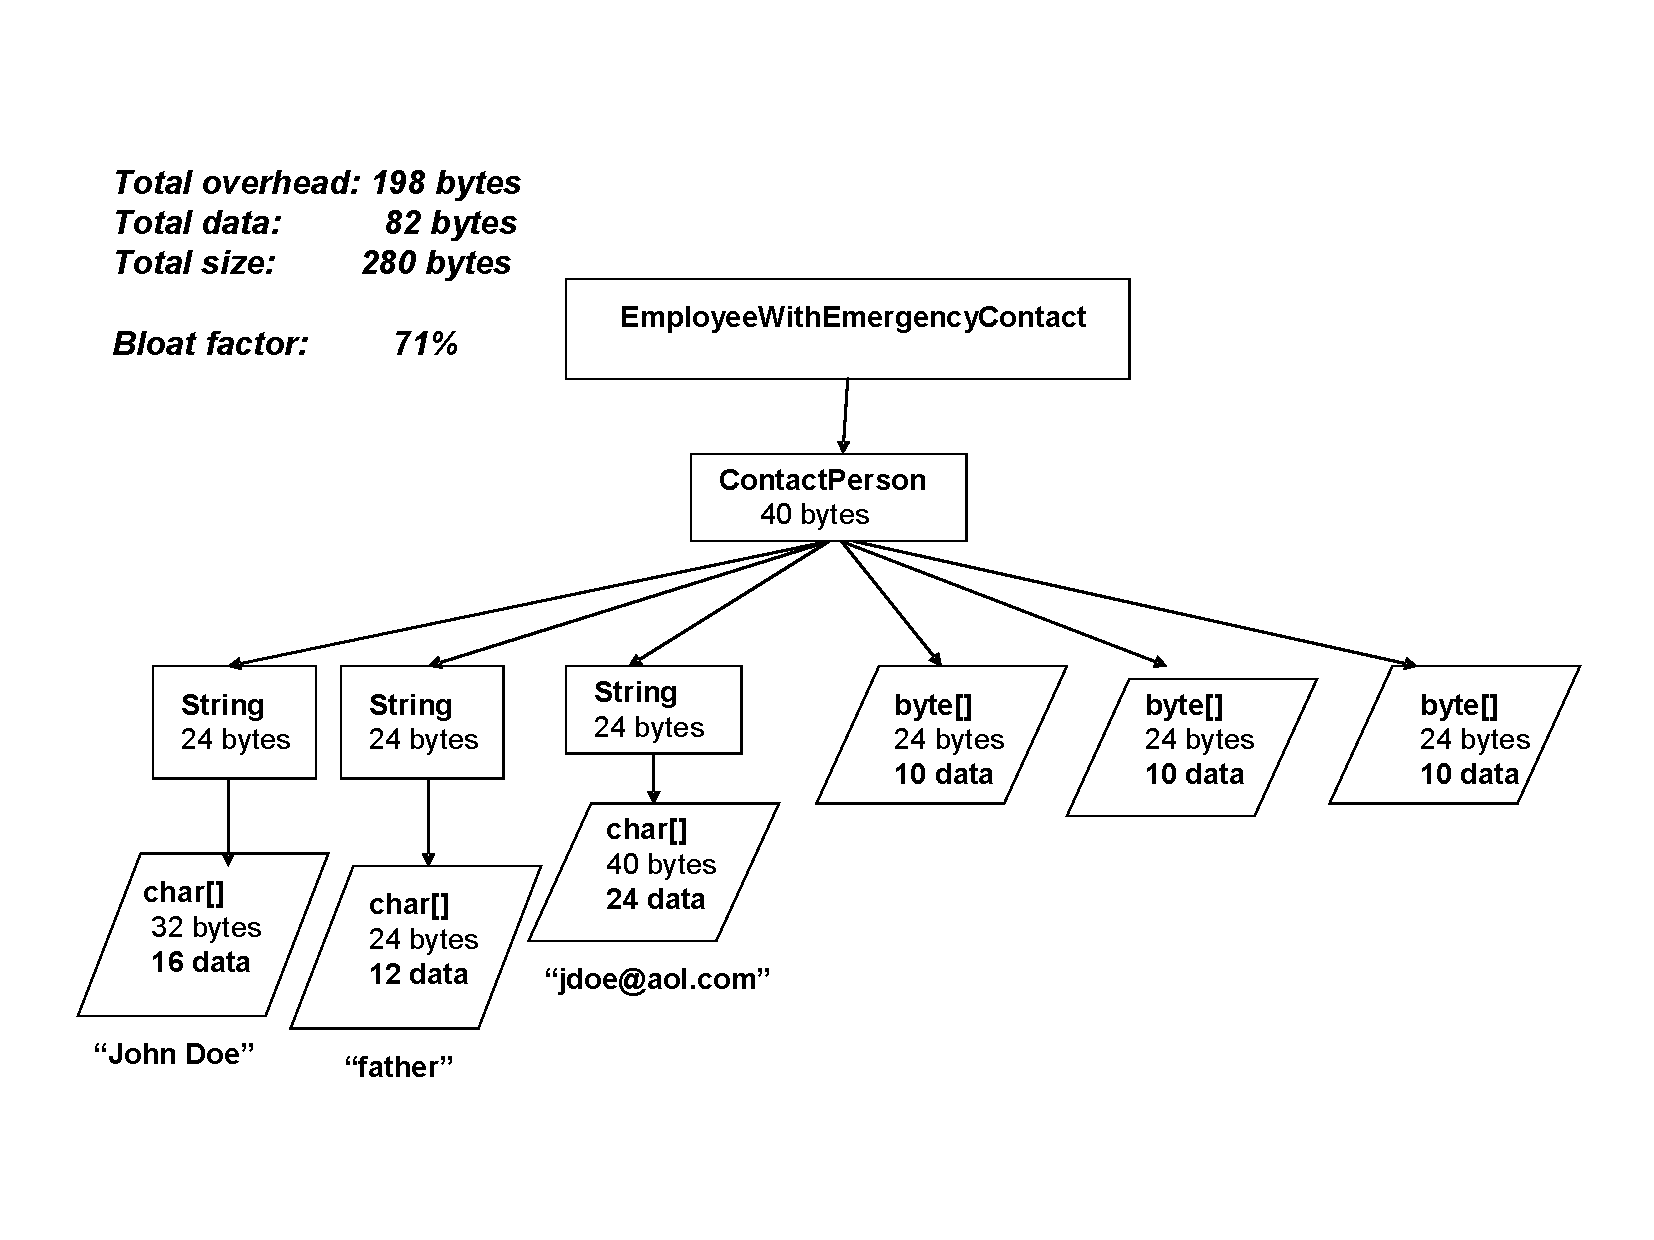
\includegraphics[width=.70\textwidth]{Figures/chapter4/refactored-fine-grain.pdf}
 % 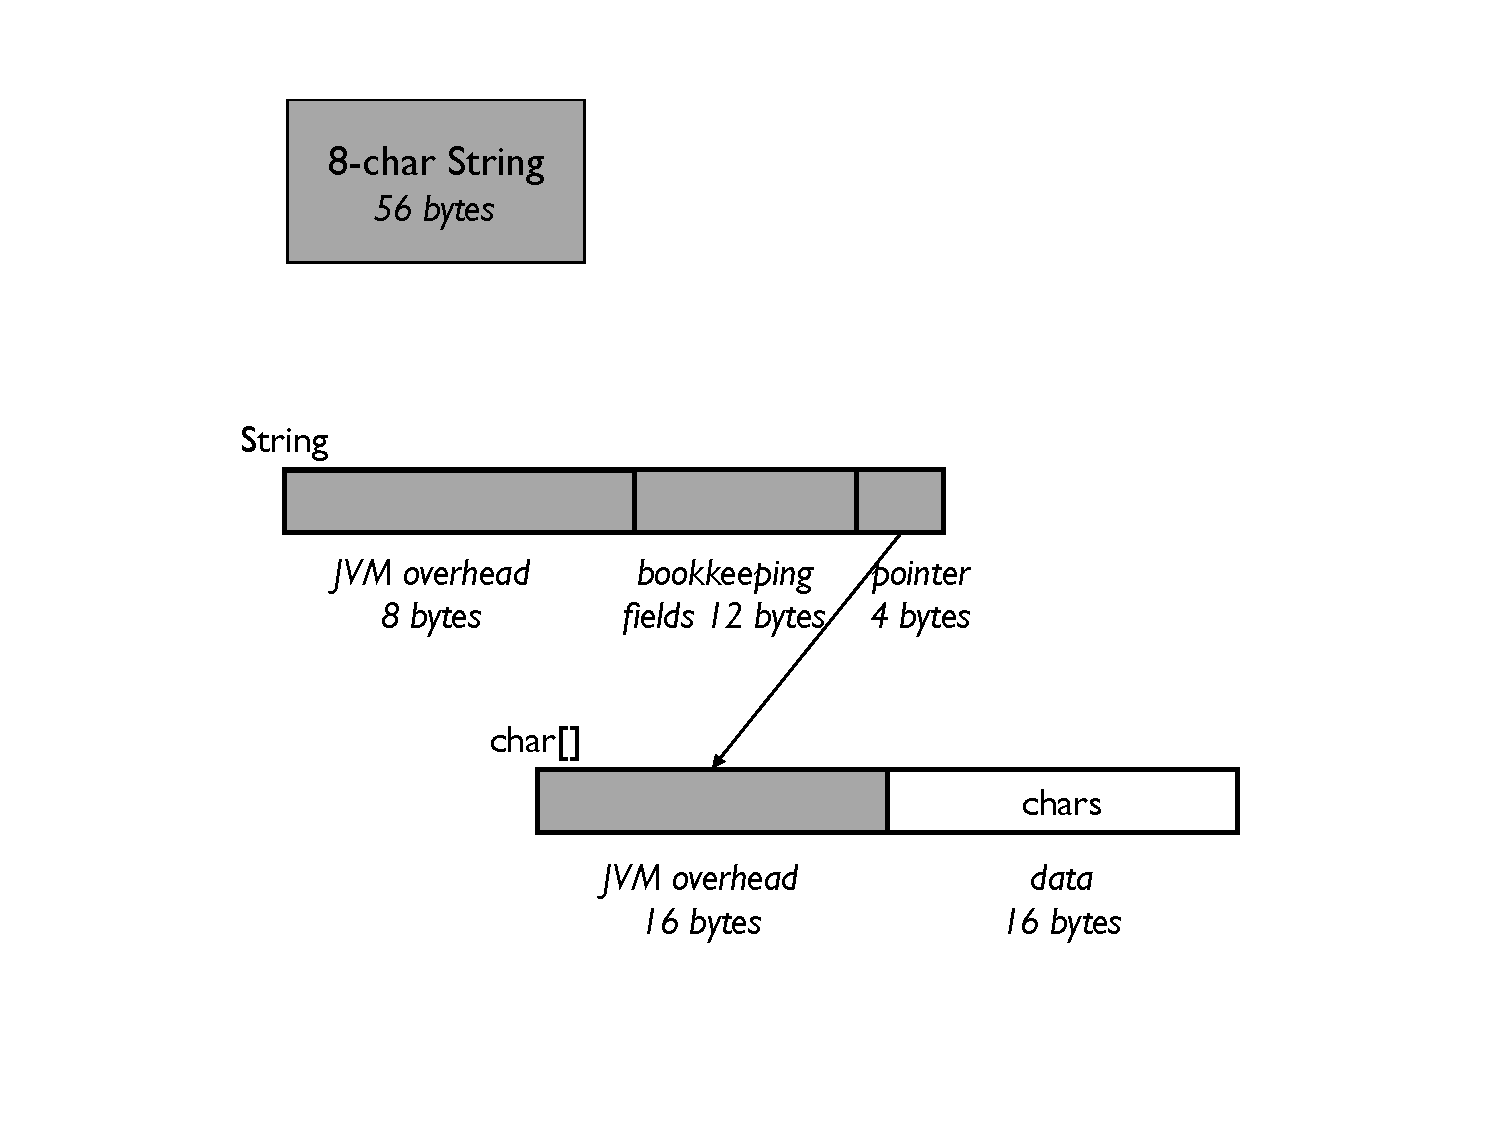
\includegraphics{eight-char-string}
  \caption{Memory layout for refactored employee emergency contact.}
  \label{fig:refactored-fine-grain}
\end{figure}

When many objects are used to represent an entity, this is an indication that the data model may be using too much delegation. Delegation is good, but it is possible to overuse a good thing. Often programmers are not aware of the overhead that delegation introduces. A design with fewer, bigger objects has less overhead and is more scalable. Whenever you use delegation, there should be a good reason. This is especially true for the important data entities in an application, those that will determine the scalability of the program.  
 
\section{Large Base Classes}

The last section discussed the costs highly-delegated data models that result in too many small objects. Occasionally, you run across a highly-delegated data model where the delegated objects are large. This can happen when delegated classes inherit from a large base class. When fine grained data modeling is combined with inheriting from large base classes, memory costs multiply and can become prohibitive. 

\begin{example}[Keeping track of updates] 

A frequent data management requirement is to track creation and update information, that is, when data is created or updated and by whom.  Here is a base class, taken from a real application, that stores create and update information.  
\ttfamily
\begin{verbatim}
      class UpdateInfo {
         Date createDate;
         Party enteredBy;
         Date updateDate;
         Party updateBy;
      }
\end{verbatim}
\normalfont
You can track changes by subclassing from \texttt{UpdateInfo}. Update tracking is a \textit{cross-cutting feature}, since it can apply to any class in a data model.

\end{example}
Returning to Example 3 in Section~\ref{fine-grained-data-models}, suppose that updates to employee emergency contacts need to be tracked. You need to decide how precise the tracking should be. Should every update to every phone number and email address be tracked, or is it sufficient to track the fact that some contact information was changed for an emergency contact? If you decide to track changes to every contact phone number or email address, you can easily achieve this by extending the \texttt{ContactMethod} class defined in the fine-grained data model from Section~\ref{fine-grained-data-models}:
\ttfamily
\begin{verbatim}
      class ContactMethod extends UpdateInfo {
         ContactPerson owner;
      }
\end{verbatim}
\normalfont
Figure~\ref{fig:big-base-class} shows an instance of an contact person with update information associated with every \texttt{ContactMethod}. Not only is this a highly delegated structure with multiple \texttt{ContactMethod} objects, but each one has an additional 16 bytes. Furthermore, there are potentially four more objects of type \texttt{Date} and \texttt{Party} for each of the four \texttt{ContactMethod} objects. A far more scalable solution is to move up a level, and track changes to each \texttt{ContactPerson}. With this solution, you do not need such a fine-grained data model, and the update tracking functionality is 1/4 the cost.
\begin{figure}
  \centering
 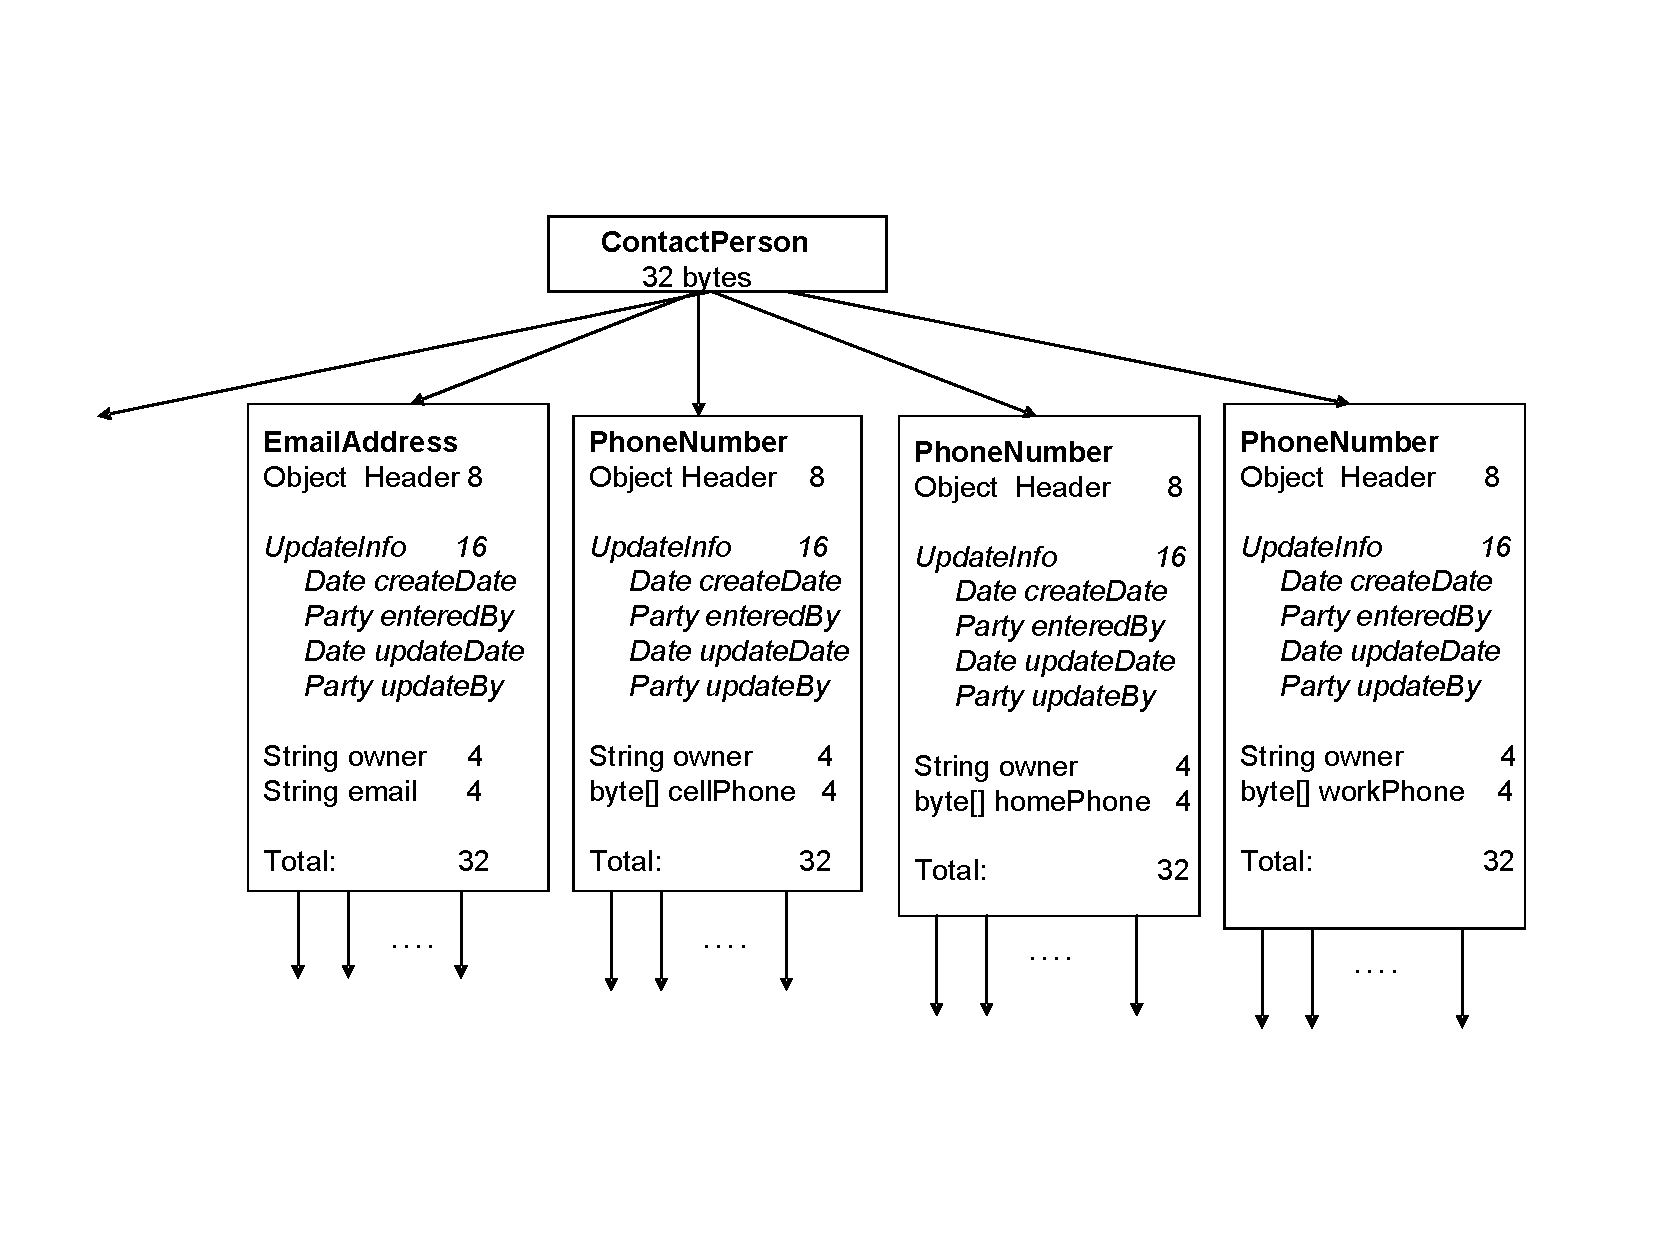
\includegraphics[width=.70\textwidth]{Figures/chapter4/big-base-class.pdf}
 % 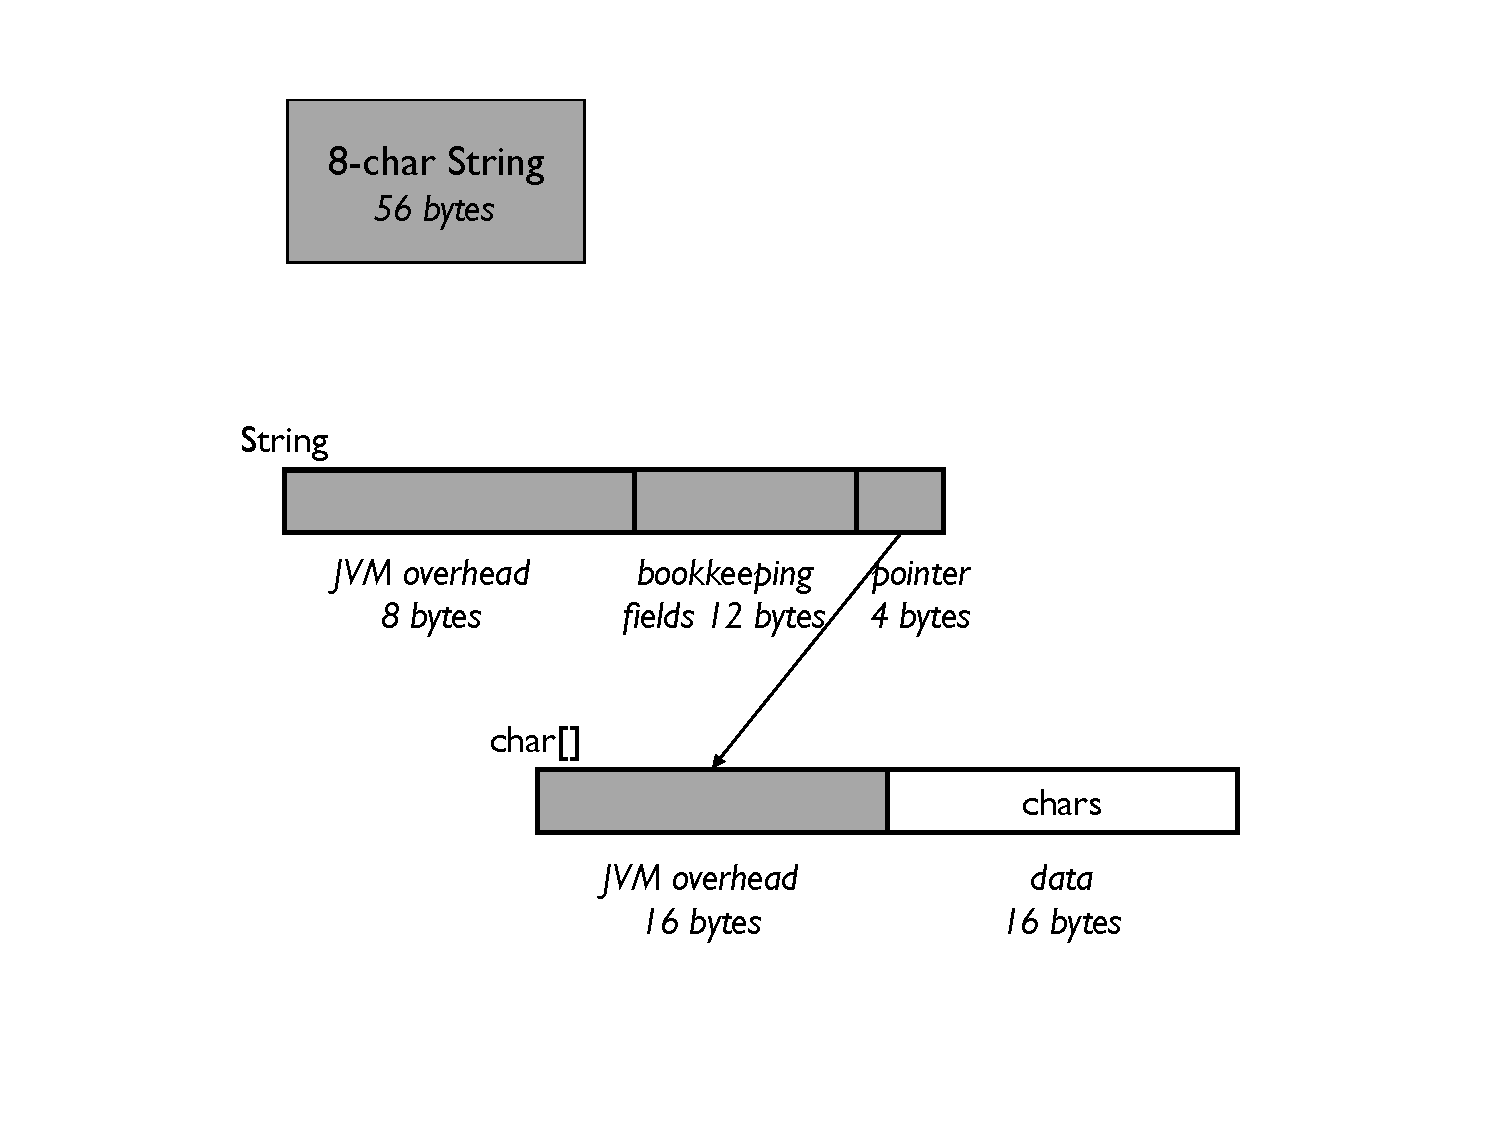
\includegraphics{eight-char-string}
  \caption{The cost of associating \texttt{UndateInfo} with every \texttt{ContactMethod}.}
  \label{fig:big-base-class}
\end{figure}
 
The solution in Figure~\ref{fig:big-base-class} provides a very fine granularity of functionality. An argument can be made in favor of this solution, since you lose functionality and flexibility if you only track updates to \texttt{ContactPerson}. However, if the program hits a scalabity problem, it may not be possible to be this casual with memory. Also, there is likely an alternate design that gives the desired functionality in a more memory-efficient way. In this example, you could implement an update log instead of tracking updates in the objects themselves. Assuming updates are sparse, this is a much better solution. Often programmers are just not aware of this potential memory problem at data model design time. It is very easy to subclass without looking closely at the memory size of a superclass, especially if the inheritance chain is long.   

\section{64-bit Architectures}

If your application does not fit into memory, perhaps moving to a 64-bit architecture will save you. However, to support a 64-bit address space, more memory is required. Object header sizes double, and pointers are 8 bytes instead of 4. Some studies~\cite{compressedAddress} show that memory consumption can increase by 40\%-50\% going from a 32-bit to a 64-bit address space for the same Java program.
\begin{example}[8-character string] 
Consider what happens to the 8-character string from Section~\ref{sec:bloat-def} in a 64-bit JVM. The memory layout is shown in Figure~\ref{fig:8-char-string-64-bit}. The 64-bit string is 50\% bigger than the 32-bit string. All of the additional cost is overhead.
\end{example} 
 \begin{figure}
  \centering
 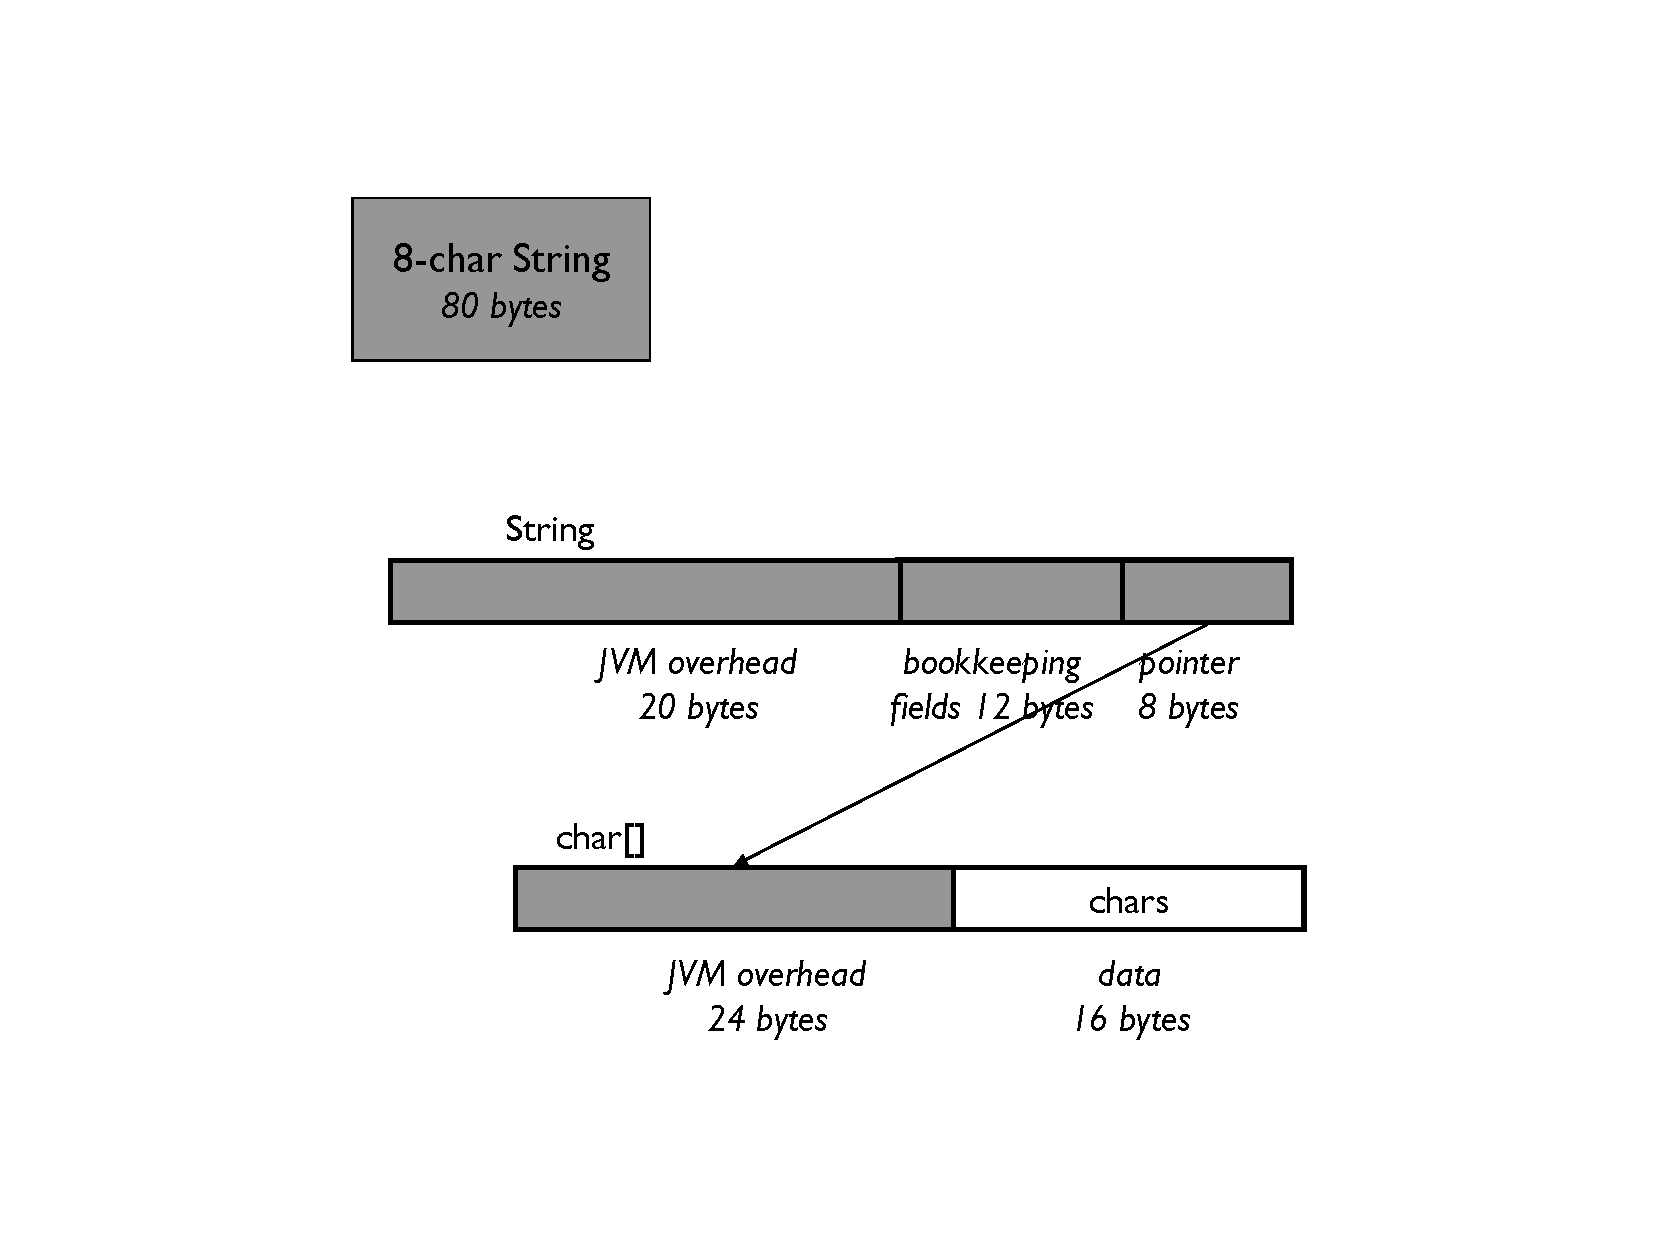
\includegraphics[width=.70\textwidth]{Figures/chapter4/8-char-string-64-bit.pdf}
 % 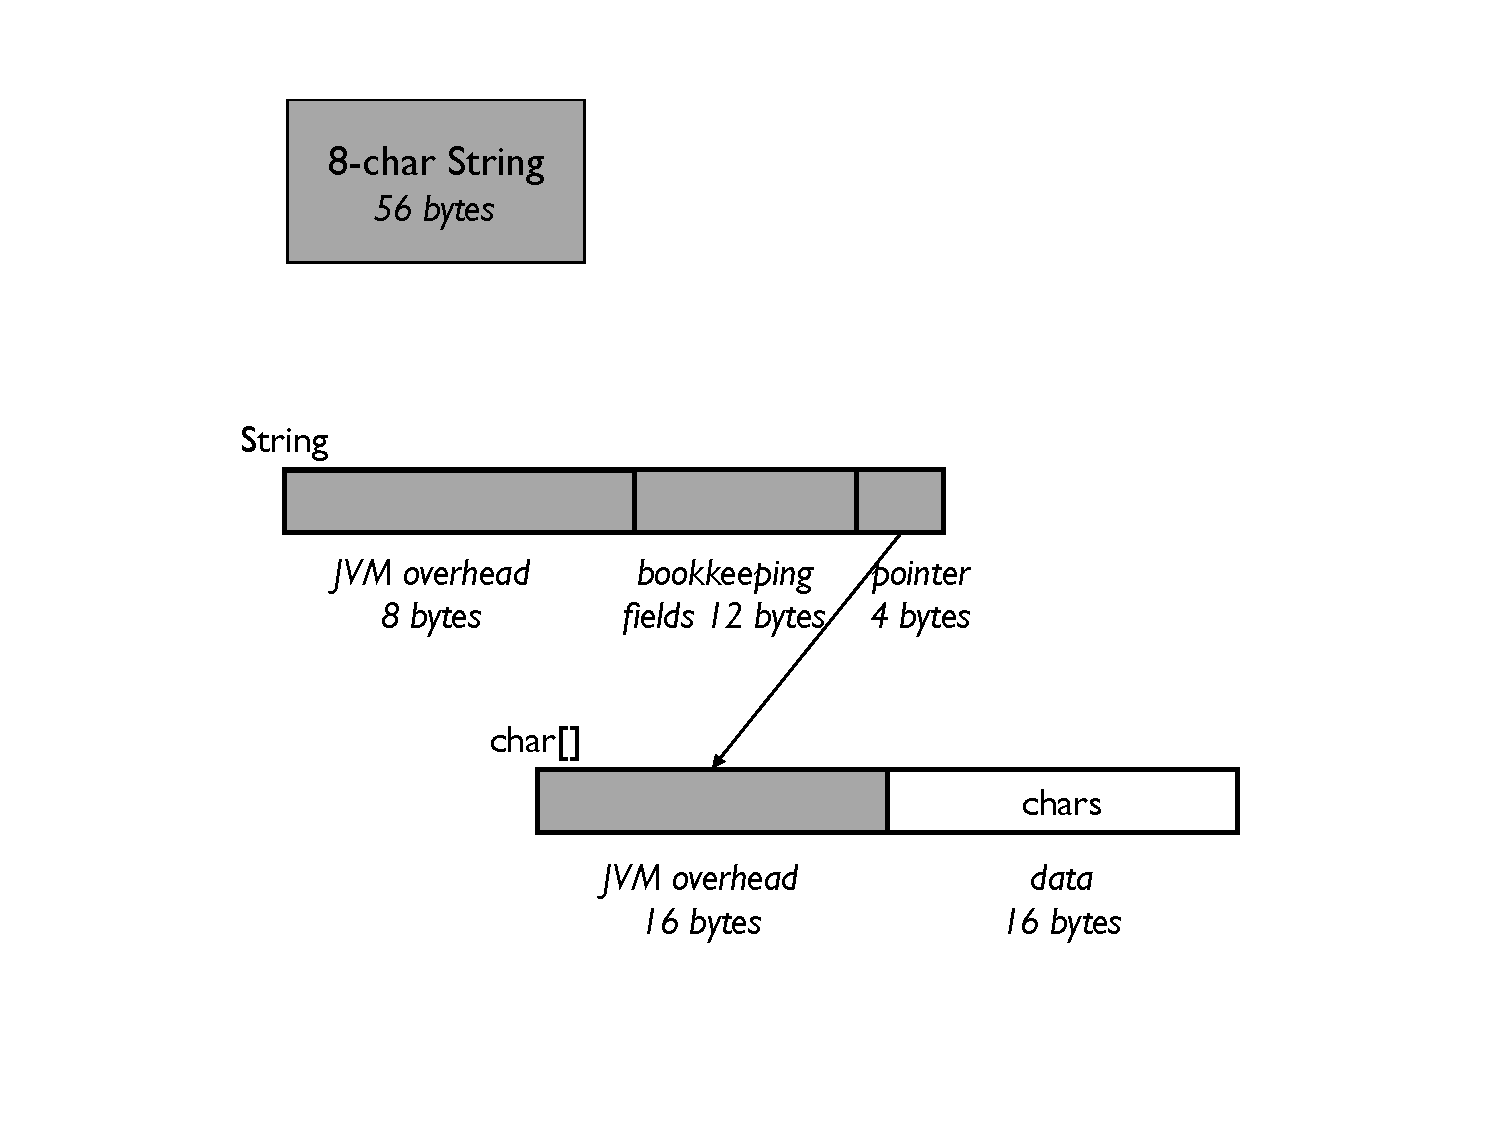
\includegraphics{eight-char-string}
  \caption{The memory layout for an 8 character string by a 64-bit JVM}
  \label{fig:8-char-string-64-bit}
\end{figure}
In reality, things are not so bad. Both the Sun and the IBM JVMs have implemented a scheme for compressing addresses that avoids this code size blowup, provided that the heap is less than 32 gigabytes. During execution, a 32-bit compressed addresses have to be converted into 64-bit native addresses, and vice-versa. 

Addess compression works as follows. A pointer stores a 4 byte offset from the base of the heap instead of an 8 byte address. The 4 byte offset added to the 64-bit base address of the heap can address any object in a 4 gigabyte byte. To achieve more compression, the offset itself is right-shifted by 3 bits. This is possible since objects are aligned on 8 byte boundaries, so the low-order 3 bits of an offset are always 0. Another 3 bits in the offset increases the address space by a factor of 8, from 4 gigabytes to 32 gigabytes. Thus, it is possible to address a 32 gigabyte heap with only 4 byte pointers.      

Address compression is available in the Sun Java 6 (update 14) release, enabled with the option -XX:+UseCompressedOops. It is available in IBM Java 6 J9 SR ???.

\section{Summary}

%An entity is modeled by a set of interrelated classes. This chapter describes how to estimate the size of an instantiated entity, using rules for estimating the size of basic objects. During the modeling process, programmers choose how many classes to define.    

Both the design of Java and software engineering best practices encourage highly delegated data models with many objects. This cost is often considered to be insignificant --- delegating to another object is just a single level of indirection. But the costs of the pointers and object headers needed to implement delegation indirection add up quickly, and contribute significantly to large bloat factors in real applications. 

The best way to evaluate whether a delegated design will scale is to identity the important classes, and measure their memory cost. This chapter describes simple rules for estimating the cost of objects, and the impact of delegation on memory overhead. Most importantly, it illustrates  the pitfalls of highly-delegated designs through examples taken from real applications.  
